% -*- Mode:TeX -*-

%% The documentclass options along with the pagestyle can be used to generate
%% a technical report, a draft copy, or a regular thesis.  You may need to
%% re-specify the pagestyle after you \include  cover.tex.  For more
%% information, see the first few lines of mitthesis.cls. 

%\documentclass[12pt,vi,twoside]{mitthesis}
%%
%%  If you want your thesis copyright to you instead of MIT, use the
%%  ``vi'' option, as above.
%%
%\documentclass[12pt,twoside,leftblank]{mitthesis}
%%
%% If you want blank pages before new chapters to be labelled ``This
%% Page Intentionally Left Blank'', use the ``leftblank'' option, as
%% above. 

\documentclass[12pt,twoside,leftblank]{mitthesis}
\usepackage{lgrind}
\pagestyle{plain}

%% in case I include .eps versions of all figures for those w/o pdftex
\usepackage{ifpdf}
\ifpdf
\usepackage[pdftex]{graphicx}
\else
\usepackage{graphicx}
\fi

\usepackage{amsmath,amssymb,amsfonts} % easily align arrays of equations
\usepackage{hyperref} % hyperlinks
\usepackage{subfig} % multi-part figures
\usepackage{pdfpages} % makes it easy to insert all those nsigmapi fits
\usepackage{multirow}
\usepackage{calrsfs} % fancier integrated luminosity script

% Feynman diagrams
\usepackage{feynmp}
\DeclareGraphicsRule{*}{mps}{*}{}

\begin{document}

\title{Measurement of Longitudinal Double Spin Asymmetries of $\pi^{+/-}$ Production in $\vec{p}+\vec{p}$ Collisions at $\sqrt{s} = 200$ GeV at RHIC}

\author{Adam Kocoloski}
\prevdegrees{B.S. Physics, University of Dayton (2004) \\
             B.A. Philosophy, University of Dayton (2004)}
\department{Department of Physics}

\degree{Doctor of Philosophy}

\degreemonth{June}
\degreeyear{2010}
\thesisdate{May 12, 2010}

\supervisor{Bernd Surrow}{Associate Professor of Physics}
\chairman{Krishna Rajagopal}{Associate Department Head for Education}

\maketitle

\cleardoublepage
% Uncomment the next line if you do NOT want a page number on your
% abstract and acknowledgments pages.
% \pagestyle{empty}
\setcounter{savepage}{\thepage}
\begin{abstractpage}
Spin dependent measurements provide incisive tests for modern theories of particle physics.  The discovery that the integral of the quark helicity distribution is much too small to account for the spin of the proton is an excellent case in point.  It inspired an intense period of theoretical scrutiny and a new generation of experiments to study \(\Delta g\), the helicity distribution of gluons in the nucleon.  In particular, the unique polarized proton collider at RHIC enables a class of asymmetry measurements that are directly sensitive to gluon polarization.

The STAR experiment at RHIC measures the double spin asymmetry \(A_{LL}\) for a variety of final states in collisions of longitudinally polarized protons in order to constrain \(\Delta g\). Asymmetries for mid-rapidity charged pion production benefit from large cross sections and the excellent tracking and particle identification capabilities of the STAR Time Projection Chamber. This thesis presents the first measurements of charged pion \(A_{LL}\) at STAR. The measurements are compared to predictions based on perturbative QCD calculations and from this comparison model-dependent constraints are placed on the integral gluon polarization \(\Delta G\).

\end{abstractpage}

% Additional copy: start a new page, and reset the page number.  This way,
% the second copy of the abstract is not counted as separate pages.
% Uncomment the next 6 lines if you need two copies of the abstract
% page.
% \setcounter{page}{\thesavepage}
% \begin{abstractpage}
% Spin dependent measurements provide incisive tests for modern theories of particle physics.  The discovery that the integral of the quark helicity distribution is much too small to account for the spin of the proton is an excellent case in point.  It inspired an intense period of theoretical scrutiny and a new generation of experiments to study \(\Delta g\), the helicity distribution of gluons in the nucleon.  In particular, the unique polarized proton collider at RHIC enables a class of asymmetry measurements that are directly sensitive to gluon polarization.

The STAR experiment at RHIC measures the double spin asymmetry \(A_{LL}\) for a variety of final states in collisions of longitudinally polarized protons in order to constrain \(\Delta g\). Asymmetries for mid-rapidity charged pion production benefit from large cross sections and the excellent tracking and particle identification capabilities of the STAR Time Projection Chamber. This thesis presents the first measurements of charged pion \(A_{LL}\) at STAR. The measurements are compared to predictions based on perturbative QCD calculations and from this comparison model-dependent constraints are placed on the integral gluon polarization \(\Delta G\).

% \end{abstractpage}

\cleardoublepage

\section*{Acknowledgments}
I am deeply indebted to all those who helped me develop the measurements
presented here. To Bernd Surrow, for his passion and his unwavering support
throughout my graduate career. To Mike Miller, Renee Fatemi, and Frank Simon,
who taught me how to think like a physicist and helped me find my place in STAR.
To Jan Balewski and Joe Seele, for advising me on the finer points of the
analysis in its closing stages, and to all of my fellow MIT RHIC Spin graduate
students, past and present, for their collaboration and occasional
commiseration. Thank you. The greater STAR Collaboration also deserves my
thanks, especially those members contributing to the spin physics program. I
won't forget Carl Gagliardi and Ernst Sichtermann's careful attention to the
detail of this analysis, nor J\'er\^ome Lauret's energetic leadership of the
Software and Computing systems on which I spent so many hours.

I want to express my gratitude to Alan Hoffman and Mike Miller for taking a
chance on starting a company with me, and for making sure that I stuck around to
finish this thesis despite all of the other demands on our time.

I owe a tremendous debt to my parents, who encouraged my inquisitiveness and
provided the kind of loving home one takes for granted when one doesn't know any
better. Thanks to them, to my brothers and sisters, to the Sulens family, my
friends back home and here in Boston, and many others.

Finally, to my wife Hillary, who has been a constant source of support and
encouragement even as she concluded her own doctoral studies and raised our
little baby girl. My greatest joy is knowing what it means to her to see this
day come to pass.


\pagestyle{plain}
\include{contents}
\begin{fmffile}{feynman-diagrams}
\chapter{Theoretical Foundations}

\section{The Simple Parton Model}

% predates QCD, invented to explain scaling of F_{1,2}
% Leader cites 69 Feynman PRL as inventor of parton model, but I skimmed the Letter and I don't see it.
% \cite{Panofsky:1968pb} -- confirmation of Bjorken scaling
% \cite{Bjorken:1968dy} -- Bjorken scaling

In the late nineteen-sixties high energy physicists at SLAC confirmed Bjorken's
hypothesis that the inelastic structure functions of the proton scaled; that is,
at high energies they did not depend on the $Q^2$ of the interaction. This
result stood in sharp contrast to the power-law behavior of the proton's elastic
form factors, and implied the existence of point-like constituents inside the
proton. These ``partons'' were conceived as effectively massless,
electromagnetically charged particles; in the deep-inelastic scattering
(DIS) regime, a virtual photon interacts with a parton, not the proton as a
whole.

Scaling is manifest when Bjorken's $F_1$ structure function is expressed in terms of the number densities $q(x)$ of quarks and $\bar q(x)$ of antiquarks as
%
\begin{equation}
  F_1(x, Q^2) = \frac{1}{2}\sum_{j}{e_j^2[q_j(x) + \bar{q}_j(x)]}
\end{equation}
%
where the sum is taken over quark flavors $j$ and $e_j$ is the electromagnetic charge of flavor $j$.  In longitudinally polarized DIS we define a polarization density $\Delta  q(x) \equiv q_+(x) - q_-(x)$ as the difference in number density between quarks whose spins are aligned with the (longitudinal) spin of the proton and quarks whose spins are anti-aligned; the polarized analogue to $F_1$ is then
%
\begin{equation}
  g_1(x, Q^2) = \frac{1}{2}\sum_{j}{e_j^2[\Delta q_j(x) + \Delta \bar{q}_j(x)]}.
\end{equation}

In the naive parton model we assume $SU(3)_F$ flavor symmetry and thus it is useful to rewrite the expression for $g_1$ in terms of quantities which have specific $SU(3)_F$ transformation properties:
%
\begin{equation}
  g_1(x) = \frac{1}{9}[\frac{3}{4}\Delta q_3(x) + \frac{1}{4}\Delta q_8(x) + \Delta \Sigma(x)]
\end{equation}
%
where
%
\begin{eqnarray}
  \Delta q_3 & = & (\Delta u + \Delta \bar{u}) - (\Delta d + \Delta \bar{d}) \nonumber \\
  \Delta q_8 & = & (\Delta u + \Delta \bar{u}) + (\Delta d + \Delta \bar{d}) - 2(\Delta s + \Delta \bar{s}) \nonumber \\
  \Delta \Sigma & = & (\Delta u + \Delta \bar{u}) + (\Delta d + \Delta \bar{d}) + (\Delta s + \Delta \bar{s})
  \label{eqn:su3_dis}
\end{eqnarray}
%
The first moments of these quantities are the hadronic matrix elements of an octet of quark $SU(3)_F$ axial-vector currents $J_{5\mu}^i$ and a flavor singlet singlet axial current $J_{5\mu}^0$.  In the limit of massless partons the non-singlet currents are conserved quantities, and are known from $\beta$-decay measurements:
%
\begin{eqnarray}
  a_3 & = & \int_0^1 dx~\Delta q_3(x) = g_A = 1.2670 \pm 0.0035 \nonumber \\
  a_8 & = & \int_0^1 dx~\Delta q_8(x) = 0.585 \pm 0.025
\end{eqnarray}
%
A measurement of the first moment of $g_1^p$ could thus be interpreted as a measurement of the singlet current $a_0 = \int_0^1 dx~\Delta \Sigma (x)$, and in turn as a measurement of the quark spin contribution to the spin of the proton.  We rearrange \ref{eqn:su3_dis} to yield an expression for $a_0$ in terms of $a_8$ and the polarized strange quark densities:
%
\begin{equation}
  a_0 = a_8 + 3 \int_0^1 dx~(\Delta s + \Delta \bar s)
  \label{eqn:a_0_prediction}
\end{equation}
%
If one assumes that the sea quark distribution is either unpolarized or CP-symmetric and thus does not contribute to the spin of the proton, Equation \ref{eqn:a_0_prediction} becomes a \textit{prediction} for $\langle S_z \rangle$, as noted by Ellis and Jaffe \cite{Ellis:1973kp} in 1974.

% Should say something about the Sehgal result \cite{Sehgal:1974rz} that concludes the quark contribution to the spin of the proton is $\sim$ 0.3, in agreement with Ellis-Jaffe but using a slightly different derivation (Bjorken sum rule \cite{Bjorken:1966jh}, equivalent parton model result (cites several people), use SU(3) symmetry to obtain same result for $\Xi^- (dss) \rightarrow \Xi^0 (uss) + e + \bar \nu_e$, expresses $\frac{G_A}{G_V}$ ratios in terms of experimentally-measurable quantities $F$ and $D$ (calls that step the octet-model results), seems that $F+D = \frac{G_A}{G_V} \approx g_A = a_3$, F/D 

% In much of the literature I see $g_A$ instead of Griffiths' $\frac{G_A}{G_V}$.  I wonder if that is a definition, or if the literature just takes the Conserved Vector Current hypothesis $G_V = 1$ for granted? -- yes, it's the latter, see Stiegler 1995

% \begin{equation}
%   \Gamma_1^p \equiv \int_0^1 dx~g_1(x) = \frac{1}{9}[\frac{3}{4}a_3 + \frac{1}{4}a_8 + a_0]
% \end{equation}

% \begin{eqnarray*}
%   a_3 \equiv g_A & = & 1.2670 \pm 0.0035 \\
%   a_8 & = & 0.585 \pm 0.025
% \end{eqnarray*}

% really should mention Bjorken's sum rule in here somewhere, since its definitely true and not model dependent
% Bjorken sum rule -- what do I need to say about it?
% \begin{equation}
%   \int_0^1 dx~g_1^p(x,Q^2) - g_1^n(x,Q^2) = \frac{g_A}{6}(1 + O(\alpha_s))
% \end{equation}

\section{First Experimental Tests}

In polarized deep inelastic scattering, a longitudinally polarized lepton beam is scattered off of nucleon targets polarized parallel or perpendicular to the beam axis. Asymmetries are formed by comparing event rates for scattering in different spin configurations.  For a spin $\frac{1}{2}$ target, the asymmetries of interest are

% Stiegler does not include the 1/2 nor the differential in this equation
\begin{equation}
  A_{\parallel} = \frac{d\sigma^{\rightarrow \Leftarrow} - d\sigma^{\rightarrow \Rightarrow}}{2d\sigma_{unpol}}, ~~~~~~~
  A_{\perp} = \frac{d\sigma^{\rightarrow \Uparrow} - d\sigma^{\rightarrow \Downarrow}}{2d\sigma_{unpol}}
\end{equation}

Spin-dependent cross sections can be calculated by contracting the elastic Compton amplitude $T_{\mu \nu}$ with the photon polarization vectors; in the presence of parity conservation and time reversal, four of these are independent \cite{??}:
%
\begin{eqnarray}
  \sigma_{1/2} & = & F_1 + g_1 - \gamma^2 g_2, \nonumber \\
  \sigma_{3/2} & = & F_1 - g_1 + \gamma^2 g_2, \nonumber \\
  \sigma_L & = & -F_1 + F_2(1+\gamma^2)/(2x),  \nonumber \\
  \sigma_{TL} & = & \sqrt{2}\gamma (g_1+g_2).
\end{eqnarray}
%
Here $\gamma^2 = Q^2/v^2$.  These four cross sections are commonly rearranged into a pair of virtual photon asymmetries $A_1$ and $A_2$:
%
\begin{equation}
  A_1 = \frac{\sigma_{1/2} - \sigma_{3/2}}{\sigma_{1/2} - \sigma_{3/2}}, ~~~~ A_2 = \frac{\sigma_{TL}}{\sigma_T}
\end{equation}
%
The longitudinal and transverse DIS asymmetries can then be written in terms of these virtual photon asymmetries,
\begin{equation}
  A_{\parallel} = D(A_1 + \eta A_2), ~~~~~ A_{\perp} = d(A_2 - \xi A_1)
\end{equation}
%
where the coefficients $D$, $\eta$, $d$, and $\xi$ can be approximated to first order in $\gamma$ in terms of the usual DIS kinematic variables and $R = \frac{\sigma_{TL}}{\sigma_T}$:
\begin{eqnarray}
  D & \approx & \frac{y(2-y)}{y^2 + 2(1-y)(1+R)}, ~~~~~~~~ \eta \approx \frac{2(1-y)}{y(2-y)} \frac{\sqrt{Q^2}}{E} \nonumber \\
  d & \approx & D \frac{\sqrt{1-y}}{1-y/2}, ~~~~~~~~ \xi \approx \gamma(1-\frac{y}{2})
\end{eqnarray}
%
$D$ can be thought of as a depolarization factor arising from the fact that the photon is not fully aligned with the lepton beam, and $\eta$, $\xi$ are kinematic factors that are usually small.  The structure functions can also be written in terms of $A_{1,2}$:
\begin{equation}
  g_1 = \frac{F_2}{2x(1+R)}(A_1+\gamma A_2), ~~~~~ g_2 = \frac{F_2}{2x(1+R)}(A_2/\gamma - A_1).
\end{equation}
Thus, measurements of $A_{\parallel}$, $A_{\perp}$, $F_2$, and $R$ are sufficient to extract the polarized structure functions of the nucleon.

% \begin{equation}
%   \gamma = \sqrt{\frac{2Mx}{Ey}}
% \end{equation}

% note that they just measured A_parallel and neglected the A_2 contribution
The first DIS experiments to extract $g_1$ were E80 and E130, conducted in the early 1980s at SLAC.  These experiments scattered longitudinally polarized electron beams off of longitudinally polarized proton targets and were able to measure $A_1^p$ in the range $0.1 < x < 0.7$.  Their results were consistent with expectations from the parton model in that limited kinematic regime.

In 1988, the European Muon Collaboration (EMC) published data on asymmetries of longitudinally polarized \textit{muon} beams scattering off of longitudinally polarized proton targets.  

From these data they extracted measurements of the proton's $g_1$ structure function over a wide range in $x$ and $Q^2$.  As shown in Figure \ref{fig:emc-g1p}, the integral value of $g_1^p$ obtained from that extraction was incompatible with the prediction from Ellis and Jaffe.

% measured asymmetry


\begin{equation}
  A_1 = (g_1 - \gamma^2 g_2)\frac{1}{F_1}, ~~~~~~~~ A_2 = \gamma(g_1+g_2)\frac{1}{F_1}
\end{equation}

\begin{figure}
  \includegraphics[width=1.0\textwidth]{figures/emc-g1p}
  \caption{EMC extraction of $g^1_p$ and its integral compared to the prediction from Ellis-Jaffe \cite{Ashman:1987hv}}
  \label{fig:emc-g1p}
\end{figure}

\begin{equation}
  A_1 \approx \frac{A_{\parallel}}{D} \approx (1 + \gamma^2)\frac{g_1}{F_1}
\end{equation}

EMC measures first moment of g1, taking a3 and a8 from beta-decay measurements means that we can extract a0 from $\Gamma_1^p$ and it's $\sim$ 0.  But

\begin{equation}
  a_0 = \Delta \Sigma = a_8 + 3(\Delta s + \Delta \bar{s})
\end{equation}

from above, and if you ignore strange quark contributions (Ellis-Jaffe) you get $a_0 \sim 0.59$, obviously in stark contrast to EMC.  This is the original ``spin crisis''.  And of course $a_0 = 2<S_z^{quarks}>$.

Any need to mention ``Cloudy Bag'' model here?  I think not.

Detailed derivation of these results can be found in \cite{Anselmino:1994gn}

\begin{equation}
  y \equiv \frac{\nu}{E} = \frac{P \cdot q}{P \cdot k}
\end{equation}

\begin{equation}
  \gamma^2 = \frac{4M^2x^2}{Q^2}
\end{equation}

\section{QCD and the improved Parton Model}

The simple parton model is a heuristic that predates the acceptance of quantum chromodynamics (QCD) as the theory of the strong interaction.  QCD introduces two important modifications to the parton model:
%
\begin{itemize}
  \item Parton density scaling is violated by a logarithmic $Q^2$ dependence.
  \item $g_1(x,Q^2)$ gains a contribution from the polarized gluon distribution in the nucleon.
\end{itemize}
%

Evolution of $g_1$: higher-order diagrams contain collinear divergences, infinities are handled by factorization which means a choice of factorization scale.  $\mu^2 = Q^2$ is the ``optimal'' choice, as a result parton densities become $Q^2$-dependent.  Dimensional regularization is ``crucial'' technique for handling collinear (and infrared?) divergences; there are ambiguities in the application of this technique for the polarized case, leading to competition between $\bar{MS}$, $AB$, and $JET$ factorization schemes ... After this, Leader jumps straight into writing down the evolution equations for the parton density functions.

\begin{equation}
  \alpha_s~ln \frac{Q^2}{m_q^2} = \alpha_s~ln \frac{Q^2}{\mu^2} + \alpha_s~ln \frac{\mu^2}{m_q^2}
\end{equation}

do i need the evolution equations and splitting functions?

gluon contribution to $g_1$:  gluonic version of Adler-Bell-Jackiw triangle diagram 

\begin{equation}
  a_0^{gluons}(Q^2) = -3 \frac{\alpha_s(Q^2)}{2\pi} \int_0^1 dx~\Delta g(x, Q^2)
\end{equation}

or you could write it as

\begin{equation}
  a_0 = \Delta \Sigma - 3 \frac{\alpha_s}{2\pi}\Delta G
\end{equation}

NB: gluon contribution to $a_0$ is zero in $\bar{MS}$ scheme.  Need to use AB or JET scheme to obtain this result.

NB: QCD is invariant under color gauge transformations, but the interpretation of individual Feynman diagrams is gauge-dependent.  The interpretation that ``looks like'' the parton model is obtained by using the light-cone gauge for the gluon vector potential.

More notes on this section from September 28:

QCD corrections to the photon-quark interaction introduce correction terms that are collinearly divergent.  These are renormalizable by factorizing into hard and soft parts.  The optimal choice of a factorization scale is $\mu^2 = Q^2$, but this means that the (soft) parton densities are now $Q^2$-dependent and perfect Bjorken scaling is broken.  However, the scaling is only logarithmic and is calculable via evolution equations.

Experiments measure $A \approx A_1 \propto g_1$.  I'm not sure how the EMC experiment establishes that relation between $A_1$ and $g_1$, though.

OK, so we have $Q^2$-dependent parton densities, and if we measure $g_1$ at multiple values of $Q^2$ for a given $x$ we can solve the evolution equation for $\Delta G$.  When we do this, are we still interpreting $g_1$ using the simple parton model formula, or do we need to include the anomalous gluon contribution too?

$g_1(x, Q^2)$ is certainly altered by the $Q^2$ evolution of the parton densities.  It becomes

\begin{equation}
  g_1(x, Q^2) = \frac{1}{2} \sum_{flavors} e_q^2 \left[\Delta q^2 + \Delta \bar{q}^2 + \frac{\alpha_s}{2 \pi} \left(\Delta C_q \otimes \Delta q + \Delta C_G \otimes \Delta G\right)\right]
\end{equation}

Depending on the factorization scheme, the first moments might not be altered by the evolution. In $\bar{MS}$ $a_3$ and $a_8$ are invariant, in $AB$ $\Delta \Sigma$ is invariant, and in $JET$ all three are.  But, just because they are independent of $Q^2$ does not mean they keep their old definitions in terms of the first moments of parton densities, does it?  I don't know.

The Adler, Bell, Jackiw triangle diagram introduces an anomalous gluonic contribution to $a_0$, and thus to the first moment of $g_1$.  This is completely separate from the $Q^2$ evolution of the parton densities.  It means that a small measured value of $a_0$ does not necessarily imply small quark polarization in the proton (this interpretation only valid in $AB$ and $JET$, because $\Delta \Sigma$ varies with $Q^2$ in $\bar{MS}$ and thus it is not appropriate to consider it as a spin).

So the question becomes, if I were to take the first moment of $g_1(x)$ as written above, would I get $\frac{1}{9}\left[\frac{3}{4}a_3+\frac{1}{4}a_8 + a_0\right]$, where $a_0$ now includes the anomalous gluonic term?  Can it be that simple?

$\Delta C_{q,G}$ are ``Wilson coefficients evaluated from the hard part calculated beyond the Born approximation'' (whatever that means).


\section{Access to $\Delta G$}

The polarized gluon density affects a affects a wide variety of observables,
and a rich experimental and computational program has developed over the past
few decades to strictly constrain it. The first experimental constraints on
\(\Delta G\) were obtained through measurements of the variation with \(Q^2\)
at fixed \(x\) of the \(g_1\) structure functions, while more recent
measurements in polarized DIS have focused on the photon-gluon fusion channel
that is directly sensitive to polarized glue. The results in this thesis rely
on a complementary and unique experimental program of polarized proton
collisions, where the partonic interactions frequently involve one or more
gluons in the initial state.

\subsection{Scaling Violations in parton densities}

Much smaller $Q^2$ lever arm than in the unpolarized case.

\begin{figure}
  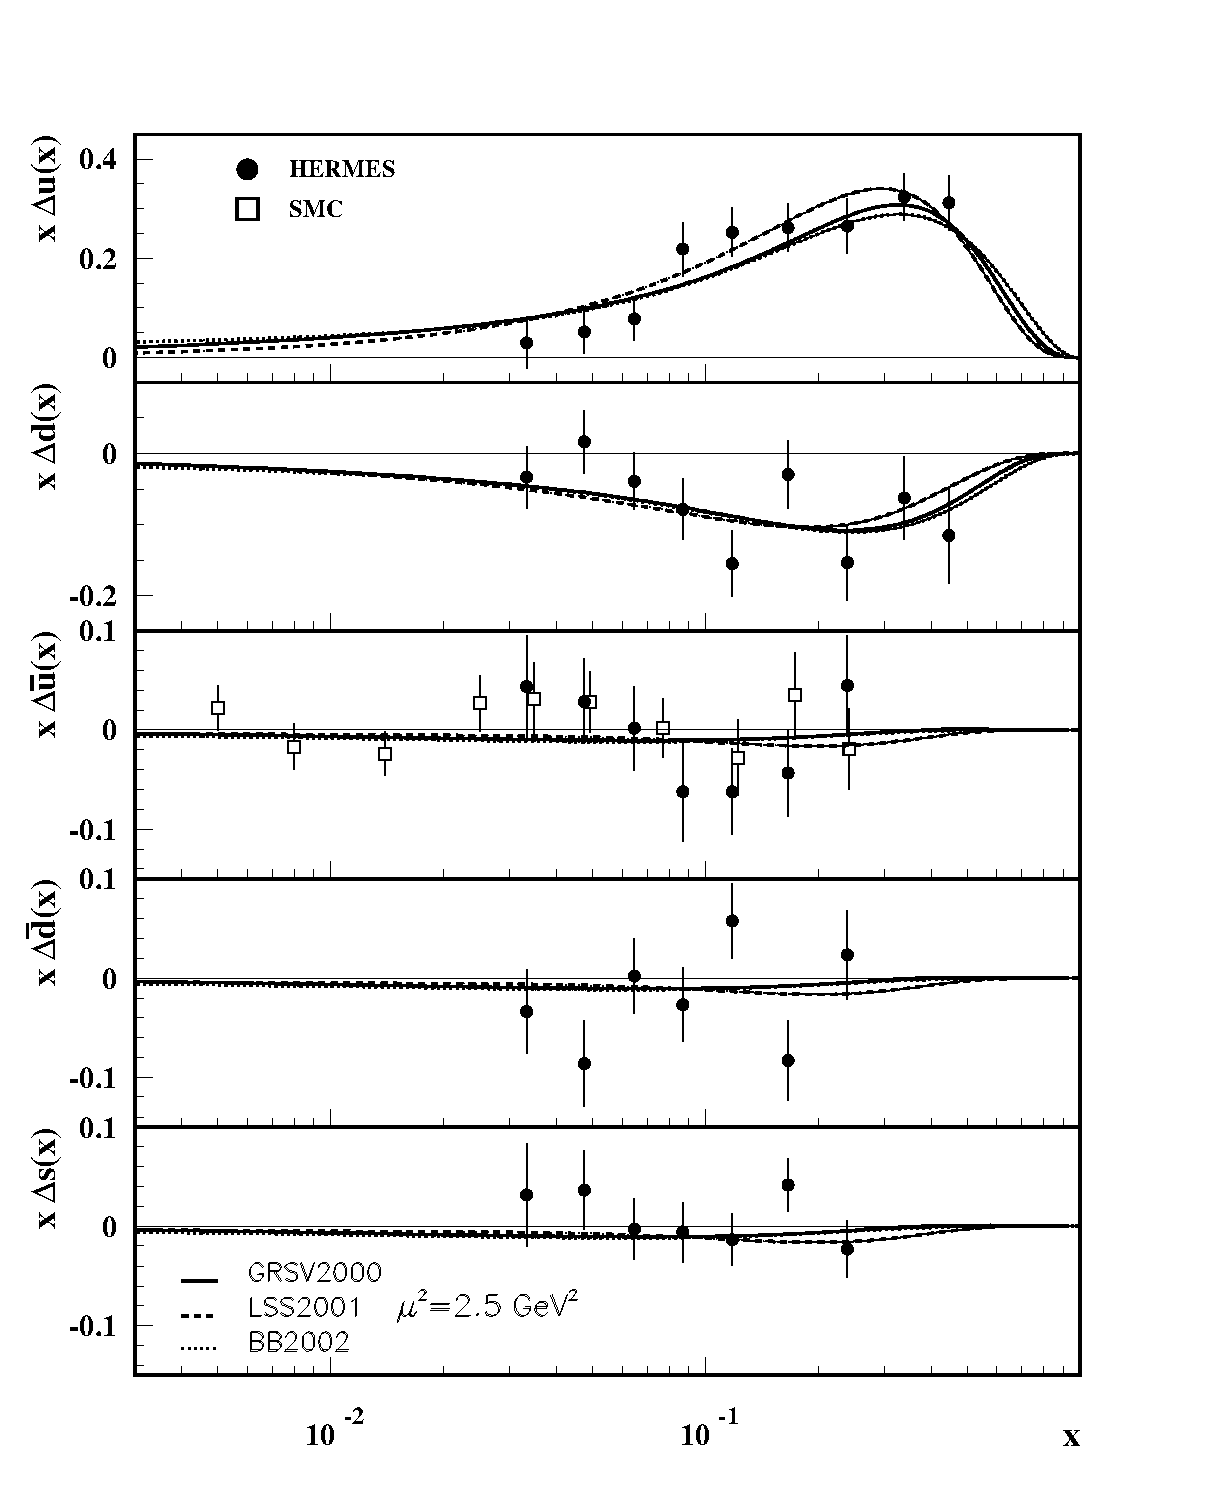
\includegraphics[width=1.0\textwidth]{figures/pol_pdf_5}
  \caption{from the Particle Data Group \cite{Amsler:2008zzb}.  Data points are SIDIS measurements using positron (HERMES) and muon (SMC).  SMC results extracted assuming $\Delta \bar u(x) = \Delta \bar d(x)$}
  \label{fig:pol_pdf_5}
\end{figure}

\begin{figure}
  \includegraphics[width=1.0\textwidth]{figures/aac03}
  \caption{\cite{Hirai:2003pm}  BB \cite{Bluemlein:2002be} uses ISET=3, LSS \cite{Leader:2001kh} uses $\bar{MS}$, GRSV \cite{Gluck:2000dy} uses STD.  But this is of course \textit{not} the most recent polarized PDF analysis using only DIS and SIDIS data.  My best guess at that is \cite{Leader:2006xc}}
\end{figure}

\begin{figure}
  \includegraphics[width=1.0\textwidth]{figures/lss06_deltag}
  \caption{Newest $\Delta g(x)$ using only DIS and SIDIS data that I'm aware of. \cite{Leader:2006xc}}
\end{figure}

Need to understand what constraints go into positive/negative/sign-changing $\Delta g(x)$ parameterizations.

\subsection{Photon-Gluon Fusion}

\begin{figure}
  \centering
  \begin{fmfgraph*}(200,150)
    \fmfleft{proton,gamma}
    \fmfright{proton',quark1,quark2}
    \fmf{fermion,width=2.5}{proton,v1}
    \fmf{fermion}{v1,proton'}
    \fmf{gluon}{v1,v2}
    \fmfblob{.15w}{v1}
    \fmf{fermion}{v2,quark1}
    \fmf{fermion}{v2,v3,quark2}
    \fmf{photon}{gamma,v3}

    % wow, it really feels like I should not have to do all of this
    \fmffixedx{0.}{v2,v3}
    \fmffixedy{0.}{v2,quark1}
    \fmffixedy{0.}{v3,quark2}
    \fmffixedy{0.}{v1,proton'}
    \fmffreeze
    \fmfshift{(0,-0.2h)}{v3}
    \fmfshift{(0.09w,-0.2h)}{quark2}
    \fmfshift{0,0.15h}{v1,proton'}
    
    % finally, add lines for outgoing quarks in struck proton
    \fmfi{plain}{vpath (__v1, __proton') shifted (thick*(-0.5,3.5))}
    \fmfi{plain}{vpath (__v1, __proton') shifted (thick*(-0.5,-3.5))}
  \end{fmfgraph*}
  \caption{Feynman diagram of photon-gluon fusion process}
\end{figure}


What's the problem with NLO analysis of these measurements?

Latest result from COMPASS analysis seems to be $\Delta g(x)/g(x) = -0.49~\pm~0.27(stat)~\pm~0.11(syst)$ at a scale $\mu^2 \sim 13 (GeV/c)^2$ and at an average gluon momentum fraction $<x>~\sim 0.11$ \cite{Alekseev:2009ey}.

%% Direct \Delta G figure without preliminary results
% \begin{figure}
%   \includegraphics[width=1.0\textwidth]{figures/compass_deltag}
%   \caption{\cite{Alekseev:2009ey}}
% \end{figure}

\begin{figure}
  \includegraphics[width=1.0\textwidth]{figures/compass_deltag_with_prelim}
  \caption{this figure comes from DIS2008, but I don't see anything in SPIRES or the arXiv on it yet.  Kurek was the author}
\end{figure}
\subsection{Polarized Proton Collisions}

``A cross section is written in factorized form as a convolution of parton distribution functions and fragmentation functions with a partonic subprocess cross section''

Assumptions:
\begin{itemize}
  \item Cross section can be written in factorized form
  \item Universality of parton distribution functions
  \item Universality of fragmentation functions
  \item partonic cross section calculable in perturbative QCD
\end{itemize}

First bullet point relies on the next 3, of course.

\begin{equation}
  A_{LL} = \frac{\sum_{f_1,f_2,f}~\Delta f_1 \otimes \Delta f_2 \otimes \sigma^{f_1 f_2 \rightarrow f X'} \hat a_{LL}^{f_1 f_2 \rightarrow f X'} \otimes D_f}{\sum_{f_1,f_2,f}~f_1 \otimes f_2 \otimes \sigma^{f_1 f_2 \rightarrow f X'} \otimes D_f} 
\end{equation}

\begin{equation}
  \hat a_{LL}^{f_1 f_2 \rightarrow f X'} = \frac{\Delta \sigma^{f_1 f_2 \rightarrow f X'}}{\sigma^{f_1 f_2 \rightarrow f X'}}
\end{equation}

\begin{figure}\begin{center}
  \includegraphics[width=0.5\textwidth]{figures/partonic_asymmetry}
  \caption{\cite{Bunce:2000uv}}
\end{center}\end{figure}


\chapter{Experimental Facilities}

\section{The Relativistic Heavy Ion Collider (RHIC)}

\begin{figure}
  \begin{center}
    \includegraphics[width=0.8\textwidth]{figures/rhic-from-above}
  \end{center}
  \caption{}
  \label{fig:rhic}
\end{figure}

The Relativistic Heavy Ion Collider (RHIC) is an intersecting storage ring located at Brookhaven National Laboratory in Upton, New York.  Unusually versatile for a collider, RHIC uses two independent superconducting rings to collide beams of ions with mass numbers separately ranging from one to 197.  Recent beam configurations have included protons on protons, deuterons on gold, copper on copper, and gold on gold.  Figure \ref{fig:rhic} shows a schematic view of the RHIC accelerator complex.  The main RHIC ring has a 3.8 kilometer circumference and is comprised of six straight sections and six curved sections.  Collisions between the beams occur in the middle of each straight section, and four experimental halls are situated at the two (BRAHMS), six (STAR), eight (PHENIX), and ten o'clock (PHOBOS) positions.

RHIC relies on a complex of smaller accelerators to prepare ion beams for injection into the main ring.  This work focuses on the systems used to polarize and accelerate beams of protons, thus avoiding further discussion of the Tandem Van de Graff generator used exclusively in heavy ion operations.  Polarized protons are produced using OPPIS \cite{Zelenski:2002gb, Zelenski:2008zza}, an optically-pumped polarized ion source which typically generates 0.5mA, 400 $\mu$s pulses of ions, corresponding to $\mathrm{9x10^{11}}$ ions per pulse.  The pulsed nature of the beam is crucial to delivering the RHIC design luminosity of $\mathrm{2x10^{32}~cm^{-2}~s^{-1}}$. OPPIS polarizes protons by passing them through a rubidium vapor pumped with circularly polarized laser light in a strong magnetic field.  The $\mathrm{H^+}$ ions pick up a polarized rubidium electron through collisions in the vapor, and magnetic fields cause the electron polarization to be transferred to the nucleus.  Finally, the hydrogen atoms are ionized to $\mathrm{H^-}$ when they pass through a sodium vapor.

The pulses of 35 keV $\mathrm{H^-}$ ions produced by OPPIS are accelerated by the LINAC, Booster, and AGS on their way to RHIC.  The LINAC strips off the electrons and accelerates the protons to a kinetic energy of 200 MeV with an efficiency of approximately 50\%.  It injects the remaining $\sim \mathrm{4x10^{11}}$ ions into the Booster ring in a single bunch.  The Booster
accelerates the protons to 1.5 GeV and passes them on to the Alternating Gradient Synchrotron (AGS), which accelerates them to the RHIC injection energy of 25 GeV.  RHIC accelerates the $\sim \mathrm{4x10^{11}}$ to the desired collision energy, which can range from 30 GeV to 250 GeV.  This work analyzes data collected with a beam energy of 100 GeV.  More details of the RHIC accelerator complex are available in references \cite{Harrison:2003sb, Hahn:2003sc, Alekseev:2003sk}.

\subsection{Spin Dynamics and Siberian Snakes}

The evolution of the spin direction of a beam of polarized protons in external magnetic fields is governed by the Thomas-BMT equation \cite{Thomas:1927yu, Bargmann:1959gz},
%
\begin{equation}
  \frac{d\vec{P}}{dt} = -\left(\frac{e}{\gamma m}\right)[(G\gamma + 1) \vec{B}_{\perp} + (G + 1) \vec{B}_{\parallel}] \times \vec{P}.
\end{equation}
%
Comparing this equation with the Lorentz force equation governing the orbital motion,
%
\begin{equation}
  \frac{d\vec{v}}{dt} = -\left(\frac{e}{\gamma m}\right)[\vec{B}_{\perp}] \times \vec{v},
\end{equation}
%
one realizes that, in a pure vertical magnetic field, the spin rotates G$\gamma$ + 1 times faster than the orbital motion. This factor, referred to as the spin tune $\nu_{sp}$, gives the number of full spin precessions for every orbit.

An accelerating beam in a storage ring encounters depolarizing resonances whenever the spin tune is equal to an integer multiple of the frequency with which a spin-depolarizing magnetic field is encountered.  In the simplest case, a depolarizing field can be introduced by a magnet error or misalignment.  For these \textit{imperfection resonances}, the resonance condition is just $G\gamma = n$.  If $G\gamma$ is non-integral, the beam sees the depolarizing field at a different point in its precession on each revolution, and the effects tend to cancel out.  The focusing fields themselves can also be a source of depolarization; for these \textit{intrinsic resonances} the resonance condition is $G\gamma = kP \pm \nu_y$, where $k$ is an integer, $\nu_y$ is the vertical betatron tune, and $P$ is the superperiodicity.

The stable spin direction in an accelerating beam normally coincides with the vertical magnetic field, but near a resonance, it gets perturbed away from the vertical by the resonance driving fields.  The polarization loss when a beam is accelerated through one of these resonances can be calculated analytically \cite{}:
%
\begin{equation}
  \frac{P_f}{P_i} = 2 e^{-\pi |\epsilon|^2 / 2\alpha} -1.
\end{equation}
%
Here $\epsilon$ is the resonance strength and $\alpha$ is the change of the spin tune per radian of the orbit angle.  When the beam is slowly accelerated ($\alpha << |\epsilon|^2$) the stable spin direction changes adiabatically and the result is a spin flip.  In contrast, techniques such as betatron tune jump serve to make $|\epsilon|^2 << \alpha$ and thus preserve the polarization through the resonance.  At high energies, the number and strength of the resonances encountered make these traditional techniques impractical.


% spin rotators

% dumping the beam

% cogging / bunch patterns

\subsection{Polarimetry Systems}

\cite{Jinnouchi:2004up} % CNI
\cite{Okada:2006dd} % H-jet

% 2 paragraphs on CNI, barely anything on H-jet

\section{The Solenoidal Tracker at RHIC (STAR)}

\cite{Ackermann:2002ad} % STAR detector overview

\begin{figure}
  \includegraphics[width=1.0\textwidth]{figures/star-schematic}
  \caption{}
  \label{fig:star-schematic}
\end{figure}

\subsection{Trigger Detectors}

\subsection{The Barrel Electromagnetic Calorimeter}

\cite{Beddo:2002zx} % BEMC overview

\subsection{The Time Projection Chamber}

\cite{Anderson:2003ur} % TPC overview

\begin{figure}
  \includegraphics[width=1.0\textwidth]{figures/tpc}
  \caption{}
  \label{fig:tpc}
\end{figure}

\subsection{Computing Facilities}

\chapter{Event Reconstruction}
\section{Detector Response Simulations}

An accurate simulation of the detector response is an important validation of a collaboration's understanding of the apparatus as well as a vital tool in the calculation of some systematic uncertainties. STAR, like many other collider experiments, uses Monte Carlo routines to generate events with properties similar to those measured by the experiment.  These events are collections of identified particles with well-defined kinematics.  STAR primarily relies on the PYTHIA 6 event generator \cite{Sjostrand:2006za} in the CDF Tune A \cite{Field:2005sa} configuration to simulate proton collisions.  A subset of results from PYTHIA have been validated using the alternative HERWIG event generator \cite{Corcella:2000bw}.  The output from PYTHIA is fed through a GEANT 3.21 \cite{GEANT321} model of the STAR detector; the end results of this process is a set of detector signals that approximate the actual detector response to a real event.  Significantly, the output from GEANT can be processed by the same reconstruction software used for real data.  Reconstruction efficiencies and other quantities useful for the estimation of systematic uncertainties can calculated by associating particles in the output of the reconstruction software with particles in the ``true'' event record generated by PYTHIA.

\section{Triggering and Data Acquisition}

STAR's proton-proton physics program stretches the capabilities of the triggering system with a rich array of algorithms and thresholds.  The basic building block of nearly all physics analyses in the 200 GeV pp program is the minimum-bias (MB) trigger, defined by coincident signals in the two BBCs.  On top of the MB trigger STAR layers a variety of requirements based on signals in the electromagnetic calorimeters that bias the event sample towards rare events with large transverse energy depositions.

The dominant trigger algorithm in this analysis is the BEMC jet patch (JP) trigger, which sums transverse energy depositions over fixed groups of 400 towers covering an area of $\Delta \eta \times \Delta \phi$ = 1.0 $\times$ 1.0.  The JP triggers were designed for efficient, minimally-biased selection of high-energy jets.  The threshold for the primary JP trigger in the 2005(2006) run was 6.4(8.3) GeV, and the integrated luminosity sampled by the trigger was ??(??) $pb^{-1}$.

\section{Tracking and Vertexing}

Tracking, the procedure by which charged particle trajectories are reconstructed from a set of detector responses, and vertexing, the determination of the position along the beam line where particles from the two beams participated in a hard scattering, are interdependent at STAR. Both rely heavily on the TPC; in this analysis the TPC is the sole tracking detector, and TPC tracks are the primary source of information used by the vertex finder.  The tracker \cite{Rose:2003wx} and vertex finder \cite{vertex-finder-starnote} aspire to
%
\begin{itemize}
  \item find tracks based on a collection of hits from the tracking detectors,
  \item fit the hits associated to a track using a suitable track model,
  \item identify an event vertex and the subset of reconstructed tracks (called primary tracks) associated with that vertex,
  \item refit the primary tracks incorporating the event vertex, and
  \item calculate final state particle information for all reconstructed tracks.
\end{itemize}
%
The wide variety of collision types analyzed at STAR present a number of challenges for the tracking and vertexing software.  Head-on (central) collisions of gold atoms can produce 6000 or more charged particles in a single event, while high luminosity proton beams can generate up to $\sim$40 ``pile-up'' collisions in the TPC volume during the 40$\mu$s drift time required to read out a single triggered bunch crossing.

STAR employs a Kalman Filter approach to combine track finding and fitting into a single process.  The essence of the Kalman approach is that the current properties of a track segment are used to define the search space for the next hit to be added to the track, and when that next hit is added, the track properties are incrementally refined incorporating the new information.  The tracker starts by identifying a track seed, a short sequence of only a few hits containing the minimum amount of information needed to estimate the track's direction and curvature.  In principle these seeds could be constructed using hits from any region of the detector, but the most effective approach is to construct them using hits from the periphery of the TPC where the hit concentration is lowest.  The Kalman search proceeds to extrapolate this track seed inward to the next active layer of the detector, in this case a TPC pad row.  Matching hits on this layer are sought within a radius determined by the errors associated with the track extrapolation.  If no matching hit is found, the extrapolation moves on to the next layer.  If one or more hits are found, the filter calculates the increase in chi-square associated with the addition of each hit to the existing track segment and chooses the hit with the lowest incremental chi-square if it falls below a configurable threshold.  Once a hit is added, the track parameters are updated using the Kalman track model and the search continues on the next detector layer.  The search terminates when it reaches the innermost layer of the detector or when it passes some number of layers without finding any matching hits.  At the culmination of the search the track parameters calculated at the innermost hit offer the best description of the track; the other nodes can be considered under-constrained because they do not incorporate information from nodes that are closer to the origin.  An outward track refit is performed to rectify this situation.  The refit updates track parameters using the same methods as the initial search; the only difference from the search is that the hits are known in advance.

On occasion a track seed is identified deeper in the TPC; in these cases, an outward extrapolation of the track is warranted, and an outward search very similar to the inward one is performed.  Once this search is complete, the inner portion of the track is refit to incorporate the information from the new outer nodes.

The tracker continues the finding and fitting procedure with new track seeds until no more seeds are found.  The tracks identified at this stage of reconstruction do not incorporate any information about the position of the event vertex and are termed ``global tracks''.  Some global tracks are pileup tracks from events other than the one that triggered the detector, some correspond to the products of strange decays in the detector, and some really are ``primary tracks'' from particles produced in the hard scattering that fired the event trigger(s).  Determining which tracks belong in each category requires a precise knowledge of the position of the event vertex, and it turns out that the best calculation of the vertex position is one that relies on the global tracks themselves.

\subsection{Vertexing}

STAR uses different vertex finders optimized for the very different running conditions of heavy ion (MinuitVF) and proton-proton (PPV) collisions.  A detailed description of both can be found in STAR Note 488 \cite{vertex-finder-starnote}; the discussion here will focus on the Pile-Up Proof Vertexer (PPV), but many of the basic principles apply to both algorithms.  

One of PPV's major design goals is robustness in the face of high levels of pileup.  Pileup events usually occur in one of the $\sim$40 other bunch crossings that are read out along with the trigger bunch crossing by the TPC, although on rare occasions a single bunch crossing can contain multiple hard scatterings.  PPV does not try to guard against this in-time pileup, but it does work to suppress false event vertices from other bunch crossings.

PPV relies on a pre-calculated beam line constraint for the $x$ and $y$ position of each vertex.  The beam line constraint is determined by running the Minuit Vertex Finder on a subset of high-multiplicity events and fitting the resulting distribution of event vertices with a straight line.  PPV uses a subset of TPC tracks satisfying a series of quality cuts; these include a transverse momentum greater than 200 MeV, a distance of closest approach (DCA) to the beam line of less than 3 cm, and a requirement that the number of hits used to fit the track is at least 70\% of the maximum number of possible hits for the track's helix.  Each track is given an initial weight based on projection of its DCA in the $xy$ plane and the errors on the extrapolation to the beam line used to calculate that DCA.  The track's weight is increased if it is reconstructed from a minimum number of hits on both sides of the central membrane of the TPC or is matched to an energy deposit in the BEMC or EEMC, since tracks satisfying one or more of those conditions are very likely to have been produced in the bunch crossing that fired the trigger(s). A track with one of these positive weight adjustments is called a ``matched'' track. Conversely, if a track extrapolates to an active calorimeter tower without any energy deposit, or crosses the central membrane but has fewer than the minimum required number of hits on both sides of the membrane, the track's weight is reduced.  The total weight for the track is the product of the initial weight and each of these adjustments.

Vertices are identified by binning the $z$ axis with 1mm resolution and generating a histogram of all the track weights.  The peak of the histogram is the first vertex candidate; all tracks which extrapolate to within 3cm of this vertex position are grouped with the candidate and removed from further analysis.  PPV iterates this procedure until no more vertex candidates can be found. In the 2005 and 2006 runs PPV required at least two ``matched'' tracks in order to save a vertex; that requirement has been relaxed in recent years to improve the vertex finding efficiency for forward triggers, which have event topologies that make it unlikely to find two tracks in an event satisfying the matching conditions.  PPV saves multiple vertices for each event, ordered by rank; in 2005 and 2006, the rank is simply the cumulative weight of all the tracks in the vertex.  The vertex finding efficiency is highly trigger-dependent; Table \ref{tbl:vertex-finding-efficiencies} lists the fraction of events with at least one primary vertex in each of the triggers used for this analysis.

\begin{table}
  \begin{center}
    \begin{tabular}{cc|ccc}
      \hline
      year & trigger ID & total events & events with vertex & efficiency\\
      \hline
      \hline
      2005 & MB (96011) & 0 & 0 & 0\\
      \hline
      2005 & BJP1 (96221) & 0 & 0 & 0\\
      \hline
      2005 & BJP2 (96233) & 0 & 0 & 0\\
      \hline
      2006 & MB (117001) & 0 & 0 & 0\\
      \hline
      2006 & BJP1 (13722[1-2]) & 0 & 0 & 0\\
      \hline
    \end{tabular}
  \end{center}
  \caption{Vertex Finding Efficiencies}
  \label{tbl:vertex-finding-efficiencies}
\end{table}

Once the vertices have been identified, the tracker adds the vertex position as an additional hit to every track associated with that vertex and refits those tracks.  The STAR software framework saves this collection of ``primary'' tracks as well as the original ``global'' tracks.  In this analysis primary tracks are used exclusively; the global tracks associated with those primaries are only analyzed to apply a more stringent cut on the DCA to the primary vertex position obtained from the original track extrapolation.

\begin{figure}
  \includegraphics[width=1.0\textwidth]{figures/ppv-candidate-distribution}
  \caption{Example vertex candidate distribution generated by PPV \cite{vertex-finder-starnote}. An ordered list of vertices is extracted from the peaks of this distribution, with the requirement that each vertex contains at least two tracks satisfying the matching conditions.}
  \label{fig:ppv-candidate-distribution}
\end{figure}

\section{Vertexing}

STAR uses different vertex finders optimized for the very different running
conditions of heavy ion (MinuitVF) and proton-proton (PPV) collisions. A
detailed description of both can be found in STAR Note 488
\cite{vertex-finder-starnote}; the discussion here will focus on the Pile-Up
Proof Vertexer (PPV), but many of the basic principles apply to both
algorithms.

One of PPV's major design goals is robustness in the face of high levels of
pileup. Pileup events usually occur in one of the $\sim$40 other bunch
crossings that are read out along with the trigger bunch crossing by the TPC,
although on rare occasions a single bunch crossing can contain multiple hard
scatterings. PPV does not try to guard against this in-time pileup, but it
does work to suppress false event vertices from other bunch crossings.

PPV relies on a pre-calculated beam line constraint for the $x$ and $y$
position of each vertex. The beam line constraint is determined by running the
Minuit Vertex Finder on a subset of high-multiplicity events and fitting the
resulting distribution of event vertices with a straight line. PPV uses a
subset of TPC tracks satisfying a series of quality cuts; these include a
transverse momentum greater than 200 MeV, a distance of closest approach (DCA)
to the beam line of less than 3 cm, and a requirement that the number of hits
used to fit the track is at least 70\% of the maximum number of possible hits
for the track's helix. Each track is given an initial weight based on
projection of its DCA in the $xy$ plane and the errors on the extrapolation to
the beam line used to calculate that DCA. The track's weight is increased if
it is reconstructed from a minimum number of hits on both sides of the central
membrane of the TPC or is matched to an energy deposit in the BEMC or EEMC,
since tracks satisfying one or more of those conditions are very likely to
have been produced in the bunch crossing that fired the trigger(s). A track
with one of these positive weight adjustments is called a ``matched'' track.
Conversely, if a track extrapolates to an active calorimeter tower without any
energy deposit, or crosses the central membrane but has fewer than the minimum
required number of hits on both sides of the membrane, the track's weight is
reduced. The total weight for the track is the product of the initial weight
and each of these adjustments.

Vertices are identified by binning the $z$ axis with 1mm resolution and
generating a histogram of all the track weights. The peak of the histogram is
the first vertex candidate; all tracks which extrapolate to within 3cm of this
vertex position are grouped with the candidate and removed from further
analysis. PPV iterates this procedure until no more vertex candidates can be
found. In the 2005 and 2006 runs PPV required at least two ``matched'' tracks
in order to save a vertex; that requirement has been relaxed in recent years
to improve the vertex finding efficiency for forward triggers, which have
event topologies that make it unlikely to find two tracks in an event
satisfying the matching conditions. PPV saves multiple vertices for each
event, ordered by rank; in 2005 and 2006, the rank is simply the cumulative
weight of all the tracks in the vertex. The vertex finding efficiency is
highly trigger-dependent; Table \ref{tbl:vertex-finding-efficiencies} lists
the fraction of events with at least one primary vertex in each of the
triggers used for this analysis.

\begin{table}
  \begin{center}
    \begin{tabular}{cc|rrr}
      \hline
      year & trigger ID & total events & events with vertex & efficiency\\
      \hline
      \hline
      2005 & MB (96011) & 1,686,762 & 1,084,203 & 64.3\%\\
      \hline
      2005 & BJP1 (96221) & 1,878,465 & 1,835,016 & 97.7\%\\
      \hline
      2005 & BJP2 (96233) & 5,446,354 & 5,243,167 & 96.3\%\\
      \hline
      2006 & MB (117001) & 257,291 & 131,657 & 51.2\%\\
      \hline
      2006 & BJP1 (13722[1-2]) & 3,294,257 & 3,138,997 & 95.3\%\\
      \hline
    \end{tabular}
  \end{center}
  \caption{Vertex Finding Efficiencies for events analyzed in this work.}
  \label{tbl:vertex-finding-efficiencies}
\end{table}

Once the vertices have been identified, the tracker adds the vertex position
as an additional hit to every track associated with that vertex and refits
those tracks. The STAR software framework saves this collection of ``primary''
tracks as well as the original ``global'' tracks. In this analysis primary
tracks are used exclusively; the global tracks associated with those primaries
are only analyzed to apply a more stringent cut on the DCA to the primary
vertex position obtained from the original track extrapolation.

\begin{figure}
  \includegraphics[width=1.0\textwidth]{figures/ppv-candidate-distribution}
  \caption{Example vertex candidate distribution generated by PPV
  \cite{vertex-finder-starnote}. An ordered list of vertices is extracted from
  the peaks of this distribution, with the requirement that each vertex
  contains at least two tracks satisfying the matching conditions.}
  \label{fig:ppv-candidate-distribution}
\end{figure}

\section{Spin Sorting}

Each of the bunches in the two RHIC beams is polarized independently, and the
polarization pattern can change from fill to fill. An accurate record of the
spin state of each bunch crossing in a fill is essential for any spin
analysis. The polarization pattern for the rings is set by the RHIC
Collider-Accelerator Department (C-AD) and broadcast through the CDEV
\cite{Barton:2003sh} control and monitoring system. The pattern is formatted
as a list of 360 8 bit numbers, one for each of the time buckets in RHIC, and
is defined in terms of the bunch crossings at the 12 o'clock position in the
RHIC ring. The beam experiences an odd number of spin flips in between 12
o'clock and the STAR IP at six o'clock, so the beam polarizations at STAR are
flipped relative to the broadcast record. The interpretation of each bit is
given in Table \ref{tbl:spin8}.

\begin{table}
  \begin{center}
  % \begin{ruledtabular}
    \begin{tabular}{c|l}
      \hline
      bit & meaning \\
      \hline
      \hline
      0 & yellow beam filled\\
      \hline
      1 & yellow beam polarized up\\
      \hline
      2 & yellow beam polarized down\\
      \hline
      3 & yellow beam unpolarized\\
      \hline
      4 & blue beam filled\\
      \hline
      5 & blue beam polarized up\\
      \hline
      6 & blue beam polarized down\\
      \hline
      7 & blue beam unpolarized\\
      \hline
    \end{tabular}
  % \end{ruledtabular}
  \end{center}
  \caption{Significance of each of the bits in an eight bit spin record.}
  \label{tbl:spin8}
\end{table}

A given bunch from the Blue ring always collides with the same bunch from the
Yellow ring at a specific interaction point in the RHIC ring over the course
of a fill. C-AD has historically configured the beams so that bunch zero from
the Blue beam collides with bunch zero from the Yellow beam at the PHENIX IP,
and as a result the PHENIX experiment sees only one abort gap in its fill
patterns. The situation is different at STAR, where the RHIC ``toggle mode''
defines the pairs of bunches from the Blue and Yellow beams that collide. The
toggle mode is typically set once at the beginning of the RHIC data-taking
period, and is encoded implicitly in the spin patterns broadcast by CDEV.

After accounting for the spin flip and the toggle mode, an analysis must map
the event IDs recorded at the experiment to the 7 bit bunch crossing IDs
defined by CDEV in order to determine the spin state of a given event. The
STAR Trigger receives this information from RHIC for every event, but analyses
have observed occasional inaccuracies in the feed that render it unreliable.
Instead, STAR uses a more robust 48 bit counter synchronized to the 9.4 MHz
RHIC clock to uniquely identify every event. The 7 bit bunch crossing IDs can
be expressed in terms of this 48 bit counter as
%
\begin{equation}
  \mathrm{7~bit~ID} = \left(\mathrm{48~bit~counter} + \mathrm{offset}\right)~mod~120
\end{equation}
%
The offset is calculated for each STAR run by generating 120 histograms of
triggers versus the 7 bit bunch IDs for each possible value of the offset,
comparing these histograms to a histogram of the intended spin pattern at
STAR, and searching for a minimum in the $\chi^2$ distribution. An example of
the overlap between the trigger rate versus bunch crossing ID and the spin
pattern after the correct offset has been applied is shown in Figure
\ref{fig:bxing-offset}. The offsets for each STAR run are calculated once and
uploaded to the STAR Calibrations DB which allows them to be applied by all
STAR spin analyses. Further details of the spin state determination can be
found in Reference \cite{spin-db-website}.

\begin{figure}
  \includegraphics[width=1.0\textwidth]{figures/bxing-offset-determined}
  \caption{Distribution of events (blue) versus the corrected 7 bit bunch
  crossing IDs at the STAR interaction point. The yellow bars indicate the
  bunch crossings where both beams have filled bunches according to the
  intended spin patterns broadcast by CDEV.}
  \label{fig:bxing-offset}
\end{figure}

\section{Jet Finding}

\subsection{Clustering Algorithm}

STAR has implemented the midpoint-cone algorithm in accordance with the recommendations of Reference \cite{Blazey:2000qt}.  The algorithm proceeds by assembling a $p_{T}$ ordered list of four momenta (``protojets") for each event.  Each protojet with $p_T>p_{T}^{seed}$ (``seeds") initiates a clustering sequence.  For each clustering sequence, protojets within an angular distance $\Delta r = \sqrt{\Delta\phi^{2} + \Delta\eta ^{2}} < r_{cone}$ are selected and their four momenta are added to define the four momentum of the cluster via $p_{\mu}^{cluster} = \sum p_{\mu}^{i}$.  If $p_{\mu}^{cluster}$ lies within a distance $\epsilon$ of the initiating protojet, the clustering sequence terminates.  Otherwise the clustering sequence is iterated about the direction $p_{\mu}^{cluster}$ until convergence is reached.  Once stable configurations are identified, the association is cataloged for later use.  However, no protojets are removed from the sample.  Clustering continues until the list of seeds is exhausted, yielding a list of redundant, overlapping, stable clusters.  Before disentangling the stable clusters, the algorithm first tests for missed initiating directions by constructing a set of test seed directions at the ``midpoint" between all possible pairs of neighboring clusters.  Specifically, locations at the midpoint of all cluster pairs separated by distance $d < 2 \times r_{cone}$ are tested for stable cluster configurations.  Clusters formed around midpoint seeds are only retained if the resulting cluster lies within $\epsilon$ of the midpoint seed, and no iteration is performed.  

After all midpoint seeds have been tested, the resulting list of stable clusters is disentangled via a splitting/merging algorithm.  The algorithm proceeds by  finding the highest $p_{T}$ cluster, referred to as the ``root" cluster.  Next, all clusters sharing protojets with the root cluster ("neighbors") are identified, and the neighbor with the largest $p_T$ is selected.  The root and neighbor jet are merged if $\frac{p_{T}^{shared}}{p_{T}^{neighbor}}>f_{split-merge}$ where $0 < f_{split-merge} < 1$.  If this condition is not satisfied the clusters are split such that each protojet is assigned to the closest of the two overlapping clusters.  After each split/merge, the cluster list is again sorted by $p_T$, a new root cluster is chosen, and the splitting/merging continues until no protojets are shared amongst clusters.  It is important to note that the split/merge step takes a  list of clusters that are essentially circular, while the final clusters are no longer necessarily circular.   Finally, each of the unique clusters is tagged as a ``jet", whose four momentum is the vector sum of the constituent protojets.

\subsection{Application at STAR}

STAR applies the midpoint-cone algorithm to cluster charged particle tracks and BEMC tower energies as follows.  Charged particle protojets are constructed from all primary TPC tracks satisfying the aforementioned cuts.  A charged pion mass is assumed when relating energy and momentum.  Each BEMC tower energy measurement is corrected for charged particle energy deposition by i) identifying the number of TPC tracks projecting to the tower and ii) subtracting the most probable MIP energy deposition for each of the projecting tracks.  After MIP subtraction, each tower energy measurement is converted to a four momentum using knowledge of the highest-ranking primary vertex location and assuming a photon mass.  Protojets are then constructed for towers with corrected $E_{T}>0.2 $GeV.   

The midpoint-cone algorithm first sorts the protojets onto a grid of $\Delta\eta=\Delta\phi=0.05$, where the properties of each grid ``cell" are defined by the vector sum of its constituent protojets.  This discretization  improves computational efficiency and minimizes potential biases arising from the fact that the BEMC towers may measure energy from more than one particle.   Each cell maintains a list of its constituent protojets so that there is no ultimate loss of information.  The midpoint cone algorithm then operates on the list of cells, and after clustering and splitting/merging conclude, each cluster is then characterized by the vector sum of its constituent four momenta.  Jets with $p_{T}<5$ GeV/$c$ are discarded.  The control parameters of the clustering algorithm are listed in Table \ref{tbl:jetfinding-parameters}.  The restricted cone radius in the 2005 analysis was motivated by the limited pseudorapidity acceptance of the partially installed BEMC.

\begin{table}
  \begin{center}
    % \begin{ruledtabular}
      \begin{tabular}{c|c|c}
      Parameter & Value & Explanation\\
      \hline \hline
      $r_{cone}$  &   0.4 (2005), 0.7 (2006) & clustering radius \\ \hline
      $p_{T}^{seed}$  &   0.5 GeV/$c$ & seed threshold \\ \hline
      $f_{split-merge}$  &  0.5  & split/merge criterion \\ \hline
      $\epsilon$  &  0.025  & clustering convergence condition \\
      \end{tabular}
    % \end{ruledtabular}    
  \end{center}
  \caption{Control parameters used in midpoint-cone clustering.}
  \label{tbl:jetfinding-parameters}
\end{table}

\section{Charged Pion Identification}

Charged pions are identified and separated from kaons, protons, and electrons by the amount of energy they lose in the TPC.  The dE/dx of a TPC track is obtained by sorting the track hits according to energy loss, removing the top 30\%, and averaging the rest.  Track dE/dx values for a given particle species at a fixed momentum are Gaussian, so one can also express the dE/dx value for each track in terms of a deviation from the mean dE/dx for some identified particle at that track's momentum.  In particular, track energy loss values at STAR are commonly given in terms of ``$n\sigma(\pi)$'', the deviation from the mean of the pion peak divided by the width of said peak.  Protons and kaons fall to the left of the pion peak (lower energy loss) and electrons fall to the right (higher energy loss).

The peak position of the raw $n\sigma(\pi)$ distribution generated by the STAR reconstruction software exhibits some significant time dependence, so instead of assuming a fixed mean of 0.0 for the pion Gaussian,  this analysis performs a triple Gaussian fit on the $n\sigma(\pi)$ distribution for each fill and extracts time-dependent means to better calibrate the PID cut.  After this recalibration one can extract yields for the various species of charged particles by fitting the $n\sigma(\pi)$ distributions with a multi-Gaussian parametric function.  The fitting procedure starts with 8 Gaussians -- one each for $\pi^{+}$, $\pi^{-}$, $K^{+}$, $K^{-}$, $p$, $\bar{p}$, $e^{+}$, and $e^{-}$.  The number of free parameters is reduced by applying the following constraints:

\begin{itemize}
    \item all widths must be equal (dE/dx resolution isn't particle-dependent)
    \item particle/antiparticle pairs should have the same mean
    \item $\pi - K$, $\pi - p$, and $\pi - e$ separations are known from other analyses \cite{Xu:2008th}
\end{itemize}

In the end there are 24 - 7 - 4 - 3 = 10 free parameters in the fit:  the Gaussian width, the position of the $\pi$ Gaussian, and the yields.  The particle separations change as a function of momentum, not $p_{T}$, so we slice a $p_{T}$ bin into momentum bins and fit each one individually.  Figure \ref{fig:typical-nsigmapi} shows a typical fit result.  The tracks have been shifted by 6*charge in order to plot positive and negatively charged tracks on the same histogram.

\begin{figure}
  \begin{center}
    \includegraphics[width=0.7\textwidth]{figures/typical-nsigmapi}    
  \end{center}
  \caption{Example PID fit result}
  \label{fig:typical-nsigmapi}
\end{figure}

With this database of particle yields in hand we can calculate the set of PID cuts that minimize the statistical uncertainty on the background-subtracted $A_{LL}$ (Equation \ref{eqn:sigma-all}).  A simple minimization routine assuming $\sigma_{A_{LL}}^{2} = 1/N$ for the raw asymmetries yields the results in Table \ref{tbl:pid-selection-windows}.

\begin{table}
    \begin{center}
        \begin{tabular}{c|ccc}
        \hline
        $p_{T}$ bin & $\pi$ window & proton/kaon max & electron min\\
        \hline
        \hline
        [2.00 - 3.18] & (-1.10, 2.30) & -2.10 & 2.60\\
        \hline
        [3.18 - 4.56] & (-1.40, 2.10) & -2.10 & 2.40\\
        \hline
        [4.56 - 6.32] & (-1.40, 1.80) & -2.10 & 2.40\\
        \hline
        [6.32 - 8.80] & (-1.40, 1.80) & -2.10 & 2.40\\
        \hline
        [8.80 - 12.84] & (-1.30, 1.40) & -2.10 & 2.10\\
    \hline
    \end{tabular}
    \end{center}
    \caption{PID Selection Windows}
    \label{tbl:pid-selection-windows}
\end{table}



\chapter{Analysis}

The analysis encompasses data taken during the 2005 and 2006 RHIC runs when
the polarized proton beams were longitudinally polarized and colliding at a
center-of-mass energy of 200 GeV. Spin asymmetries are constructed using
charged pions produced at mid-rapidity and having large transverse momentum.

\section{$A_{LL}$ Methodology}

We begin with the equation for a double spin asymmetry in terms of directly measurable quantities,
%
\begin{equation}
  A_{LL} = \frac{\sum_{runs} P_{Y}P_{B}\left[(N_{uu} + N_{dd}) - R(N_{ud} + N_{du})\right]}{\sum_{runs} P_{Y}^{2}P_{B}^{2}\left[(N_{uu} + N_{dd}) + R(N_{ud} + N_{du})\right]}.
  \label{eqn:all-basics}
\end{equation}
%
Henceforth parity conservation is employed; the \(++\) subscript denotes a sum
over the \(uu\) and \(dd\) states and the \(+-\) subscript a sum over \(ud\)
and \(du\) states. \(P_Y\) and \(P_B\) are the Yellow and Blue RHIC beam
polarizations, \(N_{ij}\) are spin-dependent charged pion yields, and \(R =
\frac{\mathcal{L}_{++}}{\mathcal{L}_{+-}}\) is a ratio of sampled luminosities
in different spin configurations. Each of the $\mathcal{L}_{ij}$ is a sum of
the scaler counts over bunch crossings with that spin state.

The formula for the statistical uncertainty on \(A_{LL}\) neglects
uncertainties on the relative luminosities and beam polarizations. Assuming
Poisson statistics on \(N_{++}\) and \(N_{+-}\) the uncertainty on the
asymmetry for a single run is
%
\begin{equation}
  \left(\frac{\sigma_{A_{LL}}}{A_{LL}}\right)^2 = \left(N_{++} + R^2 N_{+-}\right)\left[\frac{1}{N^2} + \frac{1}{D^2} - \frac{2 \times COV(N,D)}{ND} \right]
\end{equation}
%
where \(N\) and \(D\) are the numerator and denominator of the raw asymmetry
(that is, neglecting polarizations), and \(COV(N,D) = N_{++} - R^2 N_{+-}\).
In the case of small asymmetries \(\frac{1}{N^2} \gg (\frac{1}{D^2} - \frac{2
COV(N,D)}{ND}\)), and the uncertainty on the numerator dominates the uncertainty
on \(A_{LL}\):
%
\begin{equation}
  \left(\frac{\sigma_{A_{LL}}}{A_{LL}}\right)^2 \approx \frac{N_{++} + R^2 N_{+-}}{N^2}
\end{equation}
%
ROOT's TH1::Divide method does the error propagation correctly in this limit
(it ignores the covariance term). The generalization to a sum over runs is
straightforward since the yields for each run are uncorrelated.

\subsection{Multi-Particle Statistics}

This analysis often accepts multiple pions from a single event. Treating each
of the particles as an independent event and na\"ively using
$\sqrt{N_{pions}}$ for the statistical uncertainty as in the previous section
is not correct. Following the prescription in
\cite{sowinski-multiparticle-statistics} each bin in a histogram is
incremented at most once per event, using a weight equal to the number of
particles that fell into the bin. This technique neglects intra-event particle
correlations across histogram bins.

\subsection{Background Subtraction}

As discussed in Section \ref{sec:pid}, a particle's energy loss per unit path
length (dE/dx) in the TPC provides an effective means of identification across
a broad range of momenta. In the momentum range of interest (2.0 GeV/c and up)
charged pions are not fully separated from heavier charged hadrons (primarily protons and kaons, which have a smaller \(\langle dE/dx \rangle\)) and
electrons (which have a larger \(\langle dE/dx \rangle\)). This contamination is addressed by subtracting the asymmetry of
the background from the raw asymmetry calculated using all
particles in the charged pion acceptance window. The background sidebands located on both sides of the acceptance window have different physical sources and potentially different double spin asymmetries.  The subtraction
procedure must also account for the lack of a clean background sample; the
sidebands themselves have a non-negligible contamination from the charged pion
signal. We start by defining a reduced background fraction to account for the
impurities in the sideband:

\begin{equation*}
  f_{x}(y) = \frac{x~\mathrm{counts~in}~y~\mathrm{window}}{\mathrm{total~ in}~y~\mathrm{window}}
\end{equation*}

\begin{equation*}
  f'(x) = \frac{f_{x}(\pi)}{1 - f_{\pi}(x)}
\end{equation*}
%
The standard equations for the background-subtracted $A_{LL}^{\pi}$ and its
statistical uncertainty are only modified by replacing the background fraction
for each sideband with its reduced background fraction:

\begin{equation}
  A_{LL}^{\pi} = \frac{ A_{LL}^{\pi,raw} - f'(p+K)A_{LL}^{p+K,raw} - f'(e)A_{LL}^{e,raw} }{1 - f'(p+K) - f'(e)},
  \label{eqn:all}
\end{equation}

\begin{equation}
  \sigma_{A_{LL}^{\pi}} = \frac{\sqrt{ \sigma_{A_{LL}^{raw}}^{2} + f'(p+K)^{2} * \sigma_{A_{LL}^{p+K,raw}}^{2} + f'(e)^{2} * \sigma_{A_{LL}^{e,raw}}^{2} }}{1 - f'(p+K) - f'(e)}.
  \label{eqn:sigma-all}
\end{equation}
%
These equations are the final formulae used to calculate the asymmetries for a single STAR run in this work.  The \(raw\) superscript in the formulae denotes an \(A_{LL}\) calculated without background subtraction but taking multi-particle statistics into account.

Equation \ref{eqn:all-basics} specified beam polarizations, spin-dependent relative luminosities, and spin-sorted particle yields as the three components to a double spin asymmetry measurement.  A discussion of the extraction of each of these quantities follows.
\section{Beam Polarizations}

\subsection{Polarization Vectors and Transverse Asymmetries}


\section{Luminosity Determination}

Our statistical uncertainties on $A_{LL}$ assume perfect knowledge of the
relative luminosity of the different spin states. This systematic addresses
that simplification.

\subsection{Uncertainty Evaluation Using the ZDCs}

% \textit{Note: \href{http://mare.tamu.edu/star/2005n06Jets/2005relLumSys_mar29_2008/}{analysis by Murad Sarsour}}

We can quantify the precision with which we understand the relative luminosities
obtained from the BBCs by using an independent luminosity monitor, the ZDCs. In
the absence of non-statistical fluctuations, the uncertainty on R will be
dominated by the statistics in the ZDCs, which count at a much lower rate than
the BBCs during proton-proton running.

A couple of problems in the ZDC data need to be corrected before a comparison
to the BBCs can be trusted. The first problem is due to the ``killer bit''
algorithm, which suppressed signals in the ZDCs for 10 bunch crossings after
an initial signal. The algorithm is used in heavy ion running to prevent
ringing in the calorimeters from generating false signals, but in pp running
it biases the ZDC counts. Bunch crossings immediately following abort gaps
(where the killer bit is more likely to be off) end up with more ZDC counts
than crossings in the middle of a filled set of bunches. As a result, the
ratio of relative luminosities obtained from the ZDC and BBC will not be flat,
see Figure \ref{fig:zdctobbc6170012zoom}.

\begin{figure}
  \includegraphics[width=1.0\textwidth]{figures/ZDCtoBBC_r7138003}
  \caption{Ratio of ZDC and BBC counts versus bunch crossing.  Notice that the ratio is larger in bunch crossings immediately following abort gaps.}
  \label{fig:zdctobbc6170012zoom}
\end{figure}

The procedure developed to correct for this effect requires scaling the counts
for a given bunch crossing by a factor that takes into account the frequency
with which the previous ten bunch crossings had a signal. For the ZDC singles
rates, the formula for the corrected counts $n_{j}$ in a given bunch crossing
$j$ is
%
\begin{equation}
  n_{j}^{corrected} = n_{j} * \frac{N_{cycles}}{N_{cycles} - \sum_{i=1}^{10}n_{j-i}}
\end{equation}
%
where $N_{cycles}$ is the number of times the beam cycled through STAR in the
run. Figure \ref{fig:zdc-singles-ratio} shows the effect of applying the
correction for a sample run.

\begin{figure}
  \subfloat{
    \includegraphics[width=0.5\textwidth]{figures/ZDCtoBBC_r7133049ER}
  }
  \subfloat{
    \includegraphics[width=0.5\textwidth]{figures/ZDCtoBBC_r7133049WR}
  }
  \caption{Change in the ZDC singles rates after applying the killer bit correction.}
  \label{fig:zdc-singles-ratio}
\end{figure}

The formula to correct the ZDC coincidence counts is complicated by the need
to track the killer bits for the two detectors simultaneously. The formula for
the corrected coincidence counts $c_{j}$ given singles counts $e_{j}$ (ZCDE)
and $w_{j}$ (ZDCW) is
%
\begin{align}
  &\alpha_{j} = N_{cycles} - \sum_{i=1}^{10}c_{j-i} \notag\\
  &\beta_{j} = \sum_{i=1}^{10}(e_{j} + w_{j} - 2*c_{j}) - \sum_{i=1}^{9}\left[\frac{(e_{j}-c_{j}) * (w_{j}-c_{j})}{\alpha_{j}-(e_{j-10}-c_{j-10})} + \frac{(e_{j}-c_{j}) * (w_{j}-c_{j})}{\alpha_{j}-(w_{j-10}-c_{j-10})}\right] + ... \notag\\
  &c_{j}^{corrected} = c_{j} * \frac{N_{cycles}}{\alpha_{j} - \beta_{j}} 
\end{align}
%
and the effect of the killer bit correction on the coincidence distributions
is shown in Figure \ref{fig:coinRat6143016}

\begin{figure}
  \begin{center}
    \includegraphics[width=0.6\textwidth]{figures/coinRat6143016}
  \end{center}
  \caption{Change in the ZDC coincidence rates after applying the killer bit
  correction.}
  \label{fig:coinRat6143016}
\end{figure}

\begin{figure}
  \begin{center}
    \includegraphics[width=0.8\textwidth]{figures/c7308}
  \end{center}
  \caption{Example of a coherent spin pattern and even-odd ZDC rate
  oscillation. In this case, the ZDC rate is always higher when the spin of
  the blue beam is down.}
  \label{fig:c7308}
\end{figure}

The second problem that we need to correct has come to be known as the
``even-odd'' effect. It turns out that the ZDC coincidence rates are often
different for even-numbered and odd-numbered bunch crossings. This oscillation
can introduce a false asymmetry if it aligns coherently with a particular spin
pattern. For instance, in Figure \ref{fig:c7308} we see that the ZDC
coincidence rates are always higher when the spin of the blue beam is down.
Figure \ref{fig:fevfod} shows the time dependence of this even-odd
oscillation, with the colors now representing individual fills. To quantify
the bias this introduces on $A_{LL}$, we can define the fractional overlap
between the even-odd ZDC oscillation and relevant portion of the spin pattern
for $A_{LL}$ using a 120 element vector $|EO\rangle = |+1,-1,+1,-1,...\rangle$
and another 120 element vector $|LL\rangle$ whose elements are 1 if the bunch
crossing is UU or DD, -1 if UD or DU, and 0 otherwise. The inner product of
these vectors measures the susceptibility of $A_{LL}$ for that spin pattern to
any even-odd oscillation.

\begin{figure}
  \includegraphics[width=1.0\textwidth]{figures/fevfod}
  \caption{Magnitude of even-odd rate asymmetry versus time.}
  \label{fig:fevfod}
\end{figure}

It turns out that $A_{LL}$ is less biased by the even-odd rate oscillation in
the ZDC than, say, the blue beam single-spin asymmetry. Figure \ref{fig:cll}
plots the fill-by-fill change in $A_{LL}$ if the ZDC is used for relative
luminosities instead of the BBC against the the product of the fractional
overlap $F \equiv \langle EO | LL \rangle$ and the magnitude of the even-odd
oscillation $S-1$. Placing a cut on $|F*(S-1)| < 0.002$ is well-motivated. For
fills without reliable ZDC information, we use Figure \ref{fig:fevfod} to
assume a conservative $|S-1| = 0.03$.

\begin{figure}
  \begin{center}
  \includegraphics[]{figures/cll}
  \end{center}
  \caption{Change in $A_{LL}$ versus the product of the even-odd rate oscillation amplitude and the fractional overlap $\langle EO | LL \rangle$.  Deviations from 0 on the x-axis indicate fills where $A_{LL}$ is biased by the even-odd effect.}
  \label{fig:cll}
\end{figure}

After correcting for the killer bits and rejecting the fills that fail the
even-odd oscillation cut the uncertainty on $A_{LL}$ due to the uncertainty in
the relative luminosities is estimated to be $9.32\times10^{-4}$.

\subsection{Beam Background Bias}

\textit{Note: \href{http://www.star.bnl.gov/protected/spin/kowalik/2005/r-lumi/bkg_sys.html}{analysis by Kasia Kowalik}}

The relative luminosities obtained from the BBCs might also be biased by false
signals generated by beam-gas background. We can try to quantify this by
studying the coincidence rate in crossings where one of the two beams has an
unfilled bunch (``abort gaps''). The beam-gas background is assumed to be
crossing- and spin-independent, but it can be different in each beam. It
follows that the per-crossing coincidence rate due to beam-gas in each beam is
just the average number of BBC coincidences found in the abort gaps for that
beam. In Figure \ref{fig:bkg-yellow-blue}, the x-axis is the background rate
divided by the total rate, defined as the average number of coincidences per
bunch crossing with a spin state of UU, UD, DU, or DD. The two histograms are
incremented for each STAR run. We see that the background rate in the BBCs due
to beam-gas is typically less than 0.1\% of the total rate.

\begin{figure}
  \includegraphics[width=1.0\textwidth]{figures/bkg-yellow-blue}
  \caption{Fraction of the total coincidence rate attributed to beam gas in
  each beam. The histograms are incremented once for each STAR run.}
  \label{fig:bkg-yellow-blue}
\end{figure}

Given run-dependent background fractions for both beams, it's possible to
calculate background-subtracted relative luminosities. Figure
\ref{fig:r-lumi-sys-bkg} shows the difference between the raw relative
luminosity and the background-subtracted version. The background-corrected
relative luminosities yield an $A_{LL}$ that differs from the original by
$3.0\times10^{-4}$, so we use that as the uncertainty for this source of
systematic error.

\begin{figure}
  \begin{center}
    \includegraphics[width=0.6\textwidth]{figures/r-lumi-sys-bkg}
  \end{center}
  \caption{Change in the relative luminosities after correcting for beam-gas
  background.}
  \label{fig:r-lumi-sys-bkg}
\end{figure}

\input{ch4-02-data-selection}
\subsection{Trigger Bias}

STAR's BEMC jet patch trigger preferentially selects events where one of the jets is located at mid-rapidity and hadronizes with a strong electromagnetic component.  This preference indirectly biases the triggered sample toward events containing a quark jet, since quark jets have a harder fragmentation profile than gluon jets.  In addition, the jet that fires the trigger is unlikely to contain a leading charged pion.  The fragmentation bias in the trigger jet is a primary reason that our analysis of the 2006 data is restricted to pions opposite the trigger jet in azimuth.

The various biases introduced by the trigger are evaluated using a leading-order
Monte Carlo simulation of \(A_{LL}\) known as the Method of Asymmetry Weights.
Pythia supplies the kinematics and hard scattering subprocess of each simulated
event, which are sufficient to determine the partonic \(a_{LL}\) (calculated at
NLO in \cite{}). An ``asymmetry weight'' for the event is then constructed by
statistically sampling parton distribution functions:
%
\begin{equation}
  w = \frac{\Delta f_1(x_1, Q^2) * \Delta f_2(x_2, Q^2) * a_{LL}}{f_1(x_1, Q^2) * f_2(x_2, Q^2)},
\end{equation}
%
and one arrives at a Monte Carlo \(A_{LL}\) by simply taking the ratio of
asymmetry-weighted and unweighted distributions. The difference between the
\(A_{LL}\) for all Pythia events and the \(A_{LL}\) for reconstructed events
that satisfy a simulated trigger condition is used to assign the systematic
uncertainty.

\subsubsection{Monte Carlo Fragmentation Modeling}

The procedure described above requires that the Monte Carlo generator accurately reproduces the real event kinematics. Unfortunately, the fragmentation tune in Pythia~6 is not quite up to the task for STAR. Figure~\ref{fig:subprocess-fractions} is a comparison of the subprocess contributions to charged pion production reported by Pythia with the results of NLO pQCD calculations incorporating Kretzer and DSS fragmentation functions. The DSS set is known to better describe RHIC kinematics, but in Figure~\ref{fig:subprocess-fractions} it's clear that Pythia agrees much better with the Kretzer set.

\begin{figure}
  \subfloat[Kretzer]{
    \includegraphics[width=0.5\textwidth]{figures/pythia-kretzer}
    \label{fig:pythia-kretzer}
  }
  \subfloat[DSS]{
    \includegraphics[width=0.5\textwidth]{figures/pythia-dss}
    \label{fig:pythia-dss}
  }
  \caption{Comparison of subprocess contributions to charged pion production
  in Pythia and NLO pQCD calculations incorporating two different
  fragmentation functions.  The data points are results from Pythia and are the same in both plots. The Pythia results agree much better with the
  calculations using Kretzer fragmentation functions}
  \label{fig:subprocess-fractions}
\end{figure}

An accurate simulation of the subprocess contributions is an important
precondition for using the Method of Asymmetry Weights to evaluate trigger and
reconstruction bias, quite simply because $A_{LL}$ has such a strong subprocess
dependence. To confirm that the problem is really isolated to Pythia's
fragmentation functions, we examined the ratio of pions fragmenting from the
quark and the gluon in \(qg\) scattering events. That ratio is shown in Figure
\ref{fig:qg-fragmentation}, and confirms that the fragmentation model is
Kretzer-like, with much softer gluon fragmentation and/or harder quark
fragmentation than is observed at RHIC.

\begin{figure}
  \begin{center}
    \includegraphics[width=0.7\textwidth]{figures/qg-fragmentation}
  \end{center}
  \caption{Fraction of pions produced in quark-gluon scattering events that
  fragment from the gluon. Once again, the Pythia distributions agree much
  better with the calculation that uses Kretzer fragmentation functions.}
  \label{fig:qg-fragmentation}
\end{figure}

% the reweighting factor is the ratio of DSS and Kretzer FFs in each pT bin

% this reweighting factor is not applied in the 2006 analysis at the moment

Rather than plumb the depths of Pythia's independent fragmentation model, this
analysis applied a $p_{T}$- and subprocess-dependent reweighting factor to the
simulations to generate DSS-like fragmentation. The effect of this reweighting
is shown in Figure \ref{fig:compare-mcasym-nlo}. The filled markers show
markedly better agreement with the NLO pQCD calculations than the open markers,
particularly in scenarios such as GRSV-MIN where the difference in $A_{LL}$
between \(gg\) and \(qg\) subprocesses is large. The agreement is still not
perfect; one might speculate that Pythia gives too much weight to favored quark
fragmentation, since at high $p_{T}$ the $\pi^{-}$ asymmetries are too small
(indicating a relatively large d quark contribution) and the $\pi^{+}$
asymmetries are too large (consistent with a large u quark contribution).
However, as the trigger and reconstruction are not expected to be quark flavor
dependent we have decided to press forward with these simulations.

\subsubsection{2005 Bias Calculations}

\begin{figure}
  \includegraphics[width=\textwidth]{figures/compare-mcasym-nlo}
  \caption{Comparison of Monte Carlo asymmetries with NLO pQCD calculations
  incorporating DSS fragmentation functions. The open markers show results
  obtained using STAR's Pythia tune. The filled markers show the change in the
  asymmetries after reweighting the gg, qg, and qq distributions by the ratio
  of subprocess fractions calculated using DSS and Kretzer fragmentation
  functions.}
  \label{fig:compare-mcasym-nlo}
\end{figure}

Figure \ref{fig:mcasym-diff} examines the difference between asymmetries for a
``true'' sample using untriggered events and pions pulled straight from the
Pythia record, and a ``trigger+reco'' sample where the events must satisfy the
JP2 trigger simulator and the pion kinematics are obtained from TPC track
reconstruction. In some cases, the difference between the two samples is smaller
than the uncertainty on the ``trigger+reco'' sample (see Figure
\ref{fig:mcasym-sigma}). The systematic is assigned as the larger of the
difference in central values and the uncertainty on the ``trigger+reco'' sample.

The size of the systematic obviously depends on the polarized gluon
distributions that are included in the analysis. Previous measurements have
excluded the maximal polarization scenarios as well as scenarios with the
functional form of the GRSV set and integral gluon polarizations larger than 0.3
at \(Q^2 = 1 GeV^2\). As a result, we use an envelope defined by the GRSV M030
and P030 scenarios. The results of this analysis for the 2005 dataset are shown
in Table \ref{tbl:trig-reco-bias}.

% TODO recalculate bias systematic using M030 - P030 scenarios
% TODO better-looking plots for asymmetry difference and uncertainty

\begin{figure}
  \includegraphics[width=\textwidth]{figures/mcasym_run5_diff_rescaled}
  \caption{Difference between true and reconstructed Monte Carlo
  asymmetries after fragmentation reweighting.  The cyan and magenta curves represent polarized gluon distributions with the functional form of GRSV STD but with varying integral values for $\Delta G$.}
  \label{fig:mcasym-diff}
\end{figure}

\begin{figure}
  \includegraphics[width=\textwidth]{figures/mcasym_run5_sigma_rescaled}
  \caption{Uncertainty on reconstructed Monte Carlo asymmetries. If the
  uncertainty is larger than the difference between true and reconstructed
  asymmetries we use this to assign the systematic instead.}
  \label{fig:mcasym-sigma}
\end{figure}

\begin{table}[ht]
    \begin{center}
        \begin{tabular}{c|c|c}
        \hline
        $p_{T}$ & $\pi^{-}$ $\delta A_{LL}$ & $\pi^{+}$ $\delta A_{LL}$\\
        \hline
        2.00 - 3.18 & -0.0059 +0.0027 & -0.0061 +0.0061\\
        3.18 - 4.56 & -0.0083 +0.0072 & -0.0128 +0.0066\\
        4.56 - 6.32 & -0.0093 +0.0034 & -0.0176 +0.0101\\
        6.32 - 8.80 & -0.0072 +0.0036 & -0.0209 +0.0186\\
        8.80 - 12.84 & -0.0048 +0.0057 & -0.0152 +0.0062\\
    \hline
    \end{tabular}
    \end{center}
    \caption{2005 Trigger and Reconstruction Bias Uncertainties}
    \label{tbl:trig-reco-bias}
\end{table}

\subsubsection{2006 Bias Calculations}

An additional complication for the 2006 data analysis is shown in Figure~\ref{fig:mean-pt-simu}.  The JP trigger efficiency is a sharply-rising function of jet \(p_T\); as a result, the \(\langle p_T \rangle\) for pions and especially for jets in a given \(z\) bin is significantly larger in the triggered sample compared to the minimum-bias sample.  In effect, we are under-sampling the low \(x\) regime in each \(z\) bin.  The bias calculated by a na\"ive application of the Method of Asymmetry Weights to this measurement would be unacceptably large.  Instead, we choose to publish the trigger efficiency as part of the measurement, and to rescale the minimum-bias Monte Carlo sample by that trigger efficiency.  A comparison of the simulated \(A_{LL}\) in the triggered and rescaled minimum-bias samples allows an estimate of the measurement error introduced by the trigger's subprocess bias.

\begin{figure}
  \includegraphics[width=1.0\textwidth]{figures/meanpt-by-trigger}
  \caption{Comparison of the $\langle p_T \rangle$ for MB and JP triggers ni the 2006 Monte Carlo.  Filled markers plot jet $\langle p_T \rangle$ and open markers charged pion $\langle p_T \rangle$. The JP triggered data sample has a dramatically larger jet $\langle p_T \rangle$ in each $z$ bin, which biases $A_{LL}$ towards larger values in the GRSV framework.}
  \label{fig:mean-pt-simu}
\end{figure}

Figure~\ref{fig:trigger-efficiency} plots the ratio of jet yields in the MB Monte Carlo sample and the sample that passes a simulated JP trigger.  The trigger efficiency as a function of jet \(p_T\) is well described by a cubic polynomial:
%
\begin{equation}
  \epsilon_{trigger} = 1.149 - 0.2655 * p_T   + 0.01857 * p_T^2 - 0.0003445 * p_T^3.
  \label{eqn:trigger-efficiency}
\end{equation}
%
Finally, Figure~\ref{fig:trig-bias-2006} plots the difference between the trigger sample \(A_{LL}\) and the \(A_{LL}\) calculated from the rescaled MB sample for an envelope of GRSV parameterizations with integral gluon polarization less than 0.3 at \(Q^2 = 1 GeV^2\).  A systematic uncertainty on our measured \(A_{LL}\) is assigned by taking the maximum asymmetry difference in each bin, or the uncertainty on the triggered \(A_{LL}\) if all asymmetry differences are consistent with zero.

% TODO 2006 mcasym numbers for M030-P030
% TODO reweight 2006 Monte Carlo by DSS/Kretzer ratio

\begin{figure}
  \includegraphics[width=1.0\textwidth]{figures/trigger-efficiency}
  \caption{A parameterization of the BJP1 trigger efficiency as a function of corrected jet $p_T$ established from the 2006 Monte Carlo.  This parameterization is used to factor out the trigger efficiency from the Method of Asymmetry Weights $A_{LL}$ studies, allowing those studies to focus on the subprocess bias inherent in the trigger.}
  \label{fig:trigger-efficiency}
\end{figure}

\begin{figure}
  \centering
  \includegraphics[width=0.5\textwidth]{figures/placeholder}
  \caption{Comparison of simulated asymmetries for triggered events and minimum-bias events which have been rescaled to reflect the average trigger efficiency as a function of jet $p_T$. The resulting difference is a measure of the bias introduced by the subprocess-dependence in the trigger.}
  \label{fig:trig-bias-2006}
\end{figure}

\begin{table}[ht]
    \begin{center}
        \begin{tabular}{c|c|c}
        \hline
        $z$ & $\pi^{-}$ $\delta A_{LL}$ & $\pi^{+}$ $\delta A_{LL}$\\
        \hline
        0.20 - 0.30 & 0.0 &  0.0 \\
        0.30 - 0.45 & 0.0 &  0.0 \\
        0.45 - 0.65 & 0.0 &  0.0 \\
        0.65 - 1.00 & 0.0 &  0.0 \\
    \hline
    \end{tabular}
    \end{center}
    \caption{2006 Trigger and Reconstruction Bias Uncertainties}
    \label{tbl:trig-reco-bias}
\end{table}


% \subsection{Polarization Vectors and Transverse Asymmetries}

\chapter{Results and Discussion}

We have reviewed the rich history of hadronic spin physics and
identified the need to more precisely constrain the polarized gluon
distribution. We described the experimental apparatus and the analysis
techniques used to collect and study millions of polarized proton collisions
towards that end. This chapter presents the final results of the analysis, a set
of asymmetries that are directly sensitive to polarized glue and allow a deeper
understanding of the fundamental nature of QCD in the nucleon.

\section{$A_{LL}$ for Inclusive Charged Pion Production}

Figure~\ref{fig:final-result-run5} presents the first measurement of \(A_{LL}\)
for inclusive charged pion production at the STAR experiment. The data are
plotted versus the \(p_T\) of the pion and are compared to a variety of NLO pQCD
predictions. The dashed black curve represents a prediction for \(A_{LL}\) based
on the GRSV Standard parameterization of \(\Delta g(x)\), which was derived in
2001 from a global fit to polarized DIS data. The MIN and ZERO curves correspond
respectively to maximally negative and zero gluon polarization in the nucleon.
Not shown is the fourth member of the GRSV set, corresponding to maximal gluon
polarization, which has been excluded by earlier measurements of \(A_{LL}\) in
other final-state channels (and is similarly excluded by this measurement).

The dashed magenta curve labeled GS Set C is based on a polarized gluon
distribution by Gehrmann and Stirling that has a small integral polarization in
the \(x\) range accessible to 200 GeV mid-rapidity measurements at RHIC, but in
fact has a very large polarization content at smaller values of \(x\). Future
correlation measurements and measurements at a 500 GeV center-of-mass energy
will enable STAR to test whether distribution functions of this form might
correspond to reality. Finally, the solid black curve represents a new
parameterization of \(\Delta g(x)\) by de Florian, Sassot, Stratmann, and
Vogelsang which is based on a global fit incorporating both DIS data and early
\(A_{LL}\) results from RHIC.\footnote{The measurements in this thesis are not
included in the current DSSV global fit.}

\begin{figure}[ht]
  \includegraphics[width=1.0\textwidth]{figures/final-result-run5-2}
  \caption{$A_{LL}$ for inclusive charged pion production as a function of pion $p_T$ obtained from the 2005 dataset.  The error bars represent statistical uncertainties while the gray bands display total point-to-point systematic uncertainties.  The data are compared to NLO pQCD predictions incorporating various models for $\Delta g(x)$ \cite{Gluck:2000dy, Gehrmann:1995ag, deFlorian:2008mr}.}
  \label{fig:final-result-run5}
\end{figure}

\section{$A_{LL}$ for Jet + Pion Correlations}

Shown in Figure~\ref{fig:final-result-run6} are STAR's first measurements of
\(A_{LL}\) for charged pions opposite a trigger jet. The data are plotted versus
the fragmentation variable \(z\), using the away-side trigger jet \(p_T\) as a
surrogate for the \(p_T\) of the parton from which the pion fragmented. NLO pQCD
predictions for the measurement are plotted assuming the GRSV Standard, GS Set
C, and DSSV gluon distributions discussed above. The large difference in the
predictions for \(\pi^-\) \(A_{LL}\) and \(\pi^+\) \(A_{LL}\) at high \(z\) is a
reflection of the importance of favored fragmentation in that regime. Recall
that the \(\Delta u(x)\) distribution in the proton is uniformly positive, while
the \(\Delta d(x)\) distribution is smaller and uniformly negative. At high
\(z\), where the disparity between favored and disfavored fragmentation is
large, the \(\pi^-\) \(A_{LL}\) is driven by \(d\) quark scattering and the
\(\pi^+\) by \(u\) quark scattering. Favored fragmentation is also responsible
for the very different functional forms of the MIN \(A_{LL}\) prediction for
inclusive \(\pi^-\) and \(\pi^+\) \(A_{LL}\) in
Figure~\ref{fig:final-result-run5}.

\begin{figure}[]
  \includegraphics[width=1.0\textwidth]{figures/final-result-run6-4}
  \caption{$A_{LL}$ for charged pion production opposite an identified jet from the 2006 dataset.  The data are plotted against the ratio of the pion and jet transverse momenta, here labeled using the fragmentation variable $z$.  As in Figure~\ref{fig:final-result-run5}, the error bars represent statistical uncertainties and the gray bands point-to-point systematics.  The NLO predictions are the result of a recent analysis by de Florian \cite{deFlorian:2009fw}.}
  \label{fig:final-result-run6}
\end{figure}

\begin{table}
  \centering
  \begin{tabular}{|c||c|c|c||c|c|c|}
    \hline
    \multirow{2}{*}{$p_T$} & \multicolumn{3}{c||}{$\pi^{-}$} & \multicolumn{3}{c|}{$\pi^{+}$} \\
    \cline{2-7}
    & $A_{LL}$ & Stat. Error & Syst. Error &$A_{LL}$ & Stat. Error & Syst. Error\\
    (GeV/c) & ($10^{-3}$) & ($10^{-3}$) & ($10^{-3}$) & ($10^{-3}$) & ($10^{-3}$) & ($10^{-3}$) \\
    \hline
    \hline
    2.00 - 3.18 & -5.5 & $\pm$ 6.3 & -8.2 +3.4 &  -3.3 & $\pm$ 6.1 & -2.7 +2.2\\
    3.18 - 4.56 & 1.6 & $\pm$ 9.9 & -10.4 +3.4 &  -1.5 & $\pm$ 9.5 & -15.2 +3.5\\
    4.56 - 6.32 & 0.0 & $\pm$ 15.9 & -11.2 +4.6 &  3.1 & $\pm$ 15.2 & -21.1 +6.5\\
    6.32 - 8.80 & -48.9 & $\pm$ 26.4 & -11.4 +7.3 &  -1.9 & $\pm$ 25.2 & -23.5 +7.1\\
    8.80 - 12.84 & -33.0 & $\pm$ 49.4 & -14.0 +13.2 &  -72.8 & $\pm$ 48.5 & -22.2 +16.0\\
    \hline
  \end{tabular}
  \caption{$A_{LL}$ for inclusive charged pion production.}
  \label{tab:final-2005-result}
\end{table}

\begin{table}
  \centering
  \begin{tabular}{|c||c|c|c||c|c|c|}
    \hline
    \multirow{3}{*}{$z$} & \multicolumn{3}{c||}{$\pi^{-}$} & \multicolumn{3}{c|}{$\pi^{+}$} \\
    \cline{2-7}
    & $A_{LL}$ & Stat. Error & Syst. Error &$A_{LL}$ & Stat. Error & Syst. Error\\
    & ($10^{-3}$) & ($10^{-3}$) & ($10^{-3}$) & ($10^{-3}$) & ($10^{-3}$) & ($10^{-3}$) \\
    \hline
    \hline
    0.20 - 0.30 & 2.0 & $\pm$ 9.4 & -6.1 +3.2 &  1.6 & $\pm$ 9.1 & -14.0 +4.2\\
    0.30 - 0.45 & -5.9 & $\pm$ 13.9 & -12.4 +5.2 &  -14.1 & $\pm$ 13.2 & -18.0 +7.4\\
    0.45 - 0.65 & 7.0 & $\pm$ 23.4 & -16.1 +16.1 &  24.1 & $\pm$ 21.5 & -16.3 +16.5\\
    0.65 - 1.00 & 11.6 & $\pm$ 40.4 & -14.8 +10.6 &  46.0 & $\pm$ 36.5 & -17.7 +17.7\\
    \hline
  \end{tabular}
  \caption{$A_{LL}$ for charged pions opposite a trigger jet.}
  \label{tab:final-2006-result}
\end{table}

\section{Interpretation and Future Work}

A quantitive comparison of a measurement and an associated NLO prediction is obtained by calculating the \(\chi^2\) of the measurement with respect to the prediction.  One can then report the confidence level for that model of the polarized gluon distribution, which represents the probability that a \(\chi^2\) would exceed the observed \(\hat{\chi}^2\) if the model is correct.  Table~\ref{tab:confidence-levels} lists the confidence levels for all theoretical predictions plotted in Figures~\ref{fig:final-result-run5} and \ref{fig:final-result-run6}.  The \(\chi^2\) statistics are computed using statistical and point-to-point systematic uncertainties summed in quadrature.

The data are clearly incompatible with an assumption of maximally polarized gluons.  Maximally negative gluon polarization is also excluded at the 97.9\% level.  In general, the data are consistent with previous RHIC measurements in their preference for small values of gluon polarization.

The experimental methods described in this thesis are equally applicable to recent and future data taking at STAR.  A better understanding of systematic uncertainties in measurements of charged pion \(A_{LL}\) can be obtained through detailed Monte Carlo simulations of pion fragmentation as well as tighter constraints on the jet transverse momentum scale uncertainty.  Increases in luminosity and  polarization, as well as the first collisions at \(\sqrt{s} = 500\) GeV, speak to a bright future for RHIC as the experiments continue a comprehensive investigation into the spin structure of the nucleon.

\begin{table}
  \centering
  \begin{tabular}{|l||c|c|c|c|}
    \hline
    \multirow{2}{*}{Gluon Polarization Scenario} & \multicolumn{4}{c|}{Confidence Level} \\
    \cline{2-5}
    & 2005 $\pi^-$ & 2005 $\pi^+$ & 2006 $\pi^-$ & 2006 $\pi^+$ \\
    \hline
    GRSV $\Delta g$ = g & 1.6e-06 & 2e-07 & - & - \\
    GRSV $\Delta g$ = -g & 0.016 & 0.32 & - & - \\
    GRSV $\Delta g$ = 0 & 0.52 & 0.72 & - & - \\
    GRSV STD & 0.31 & 0.41 & 0.56 & 0.13 \\
    GS Set C & 0.53 & 0.79 & 0.98 & 0.59 \\
    DSSV & 0.52 & 0.71 & 0.98 & 0.59 \\
    \hline
  \end{tabular}
  \caption{Confidence levels of fitting predictions for $A_{LL}$ based on various polarized gluon distributions to the measurements presented in this thesis.}
  \label{tab:confidence-levels}
\end{table}

\end{fmffile}
% \appendix
% \include{appendices/appa}
% \include{appendices/appb}
\begin{singlespace}
\bibliography{main}
\bibliographystyle{plain}
\end{singlespace}
\end{document}

